\chapter{Combining illumination invariance with occlusion robustness and alignment}
\label{chap:pipeline}

\section{Introduction}
%
% TODO dig up old discussions of illumination wrt basri.
% TODO dig up discussion of coefficient positivity

As introduced in Chapter \ref{chap:introduction}, SRC \cite{Wright2009-PAMI} 
achieves impressive recognition results on aligned images,
it does not deal with misalignment between the test and training
images, and it requires a rich set of illuminations in the gallery images for
good performance.  The need for proper handling of image alignment and
illumination {\em simultaneously} is illustrated by an example in Figure \ref{fig:promo}.  
The task is to
identify the girl among 20 subjects. If the test face image, obtained from
an off-the-shelf face detector, has even a small amount of registration error
against the training images (caused by mild pose, scale, or misalignment), the
sparse representation obtained using the method of \cite{Wright2009-PAMI} is no
longer informative, even if sufficient illuminations are present in the
training, as shown in Figure \ref{fig:promo} (top). Additionally, in order to
span the illuminations of a typical indoor (or outdoor) environment,
illuminations from behind the subject are needed in the training set.
Otherwise, even for perfectly aligned test images, the sparse representation
obtained using \cite{Wright2009-PAMI} will not necessarily be sparse or
informative, as shown by the example in Figure \ref{fig:promo} (middle).
Clearly, both good alignment and sufficient training images are needed
to ensure success of the sparsity-based recognition method proposed by
\cite{Wright2009-PAMI}.  This chapter demonstrates a system for handling alignment
and illumination simultaneously in the sparse representation framework,
bringing the method proposed in \cite{Wright2009-PAMI} closer to practical use.

\newcommand{\tempheight}[0]{1.1in}
\begin{figure}
\centering \begin{tabular}{cc}
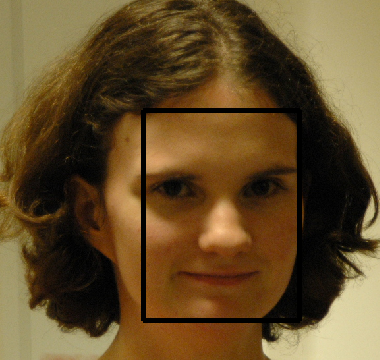
\includegraphics[height=\tempheight]{figures_pami/promo/case1/detector.png}&
\hspace{3mm}
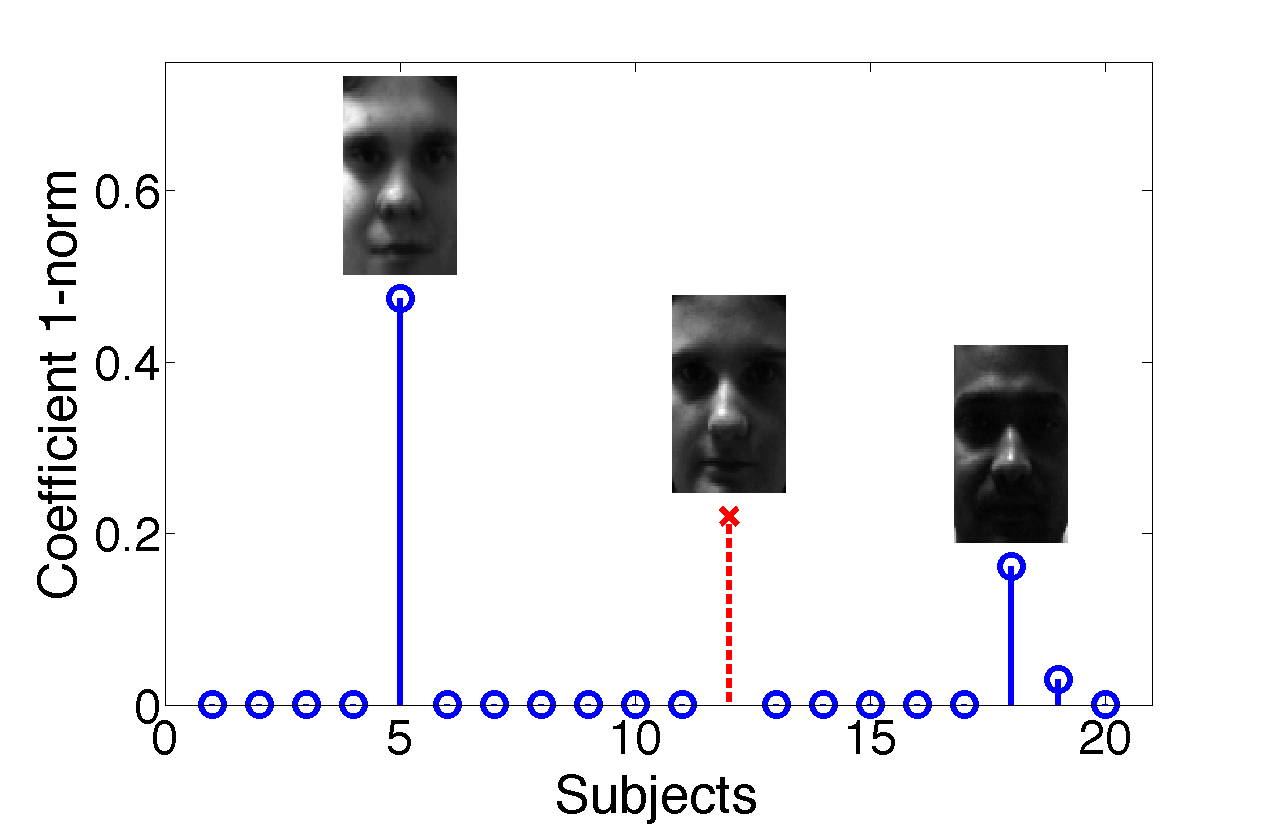
\includegraphics[height=\tempheight]{figures_pami/promo/case1/sci_with_axis_face_case1.png}
\\ 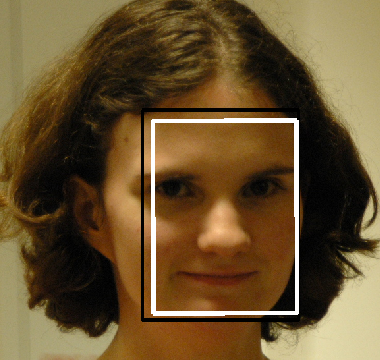
\includegraphics[height=\tempheight]{figures_pami/promo/alignment_and_detector.png}&
\hspace{3mm}
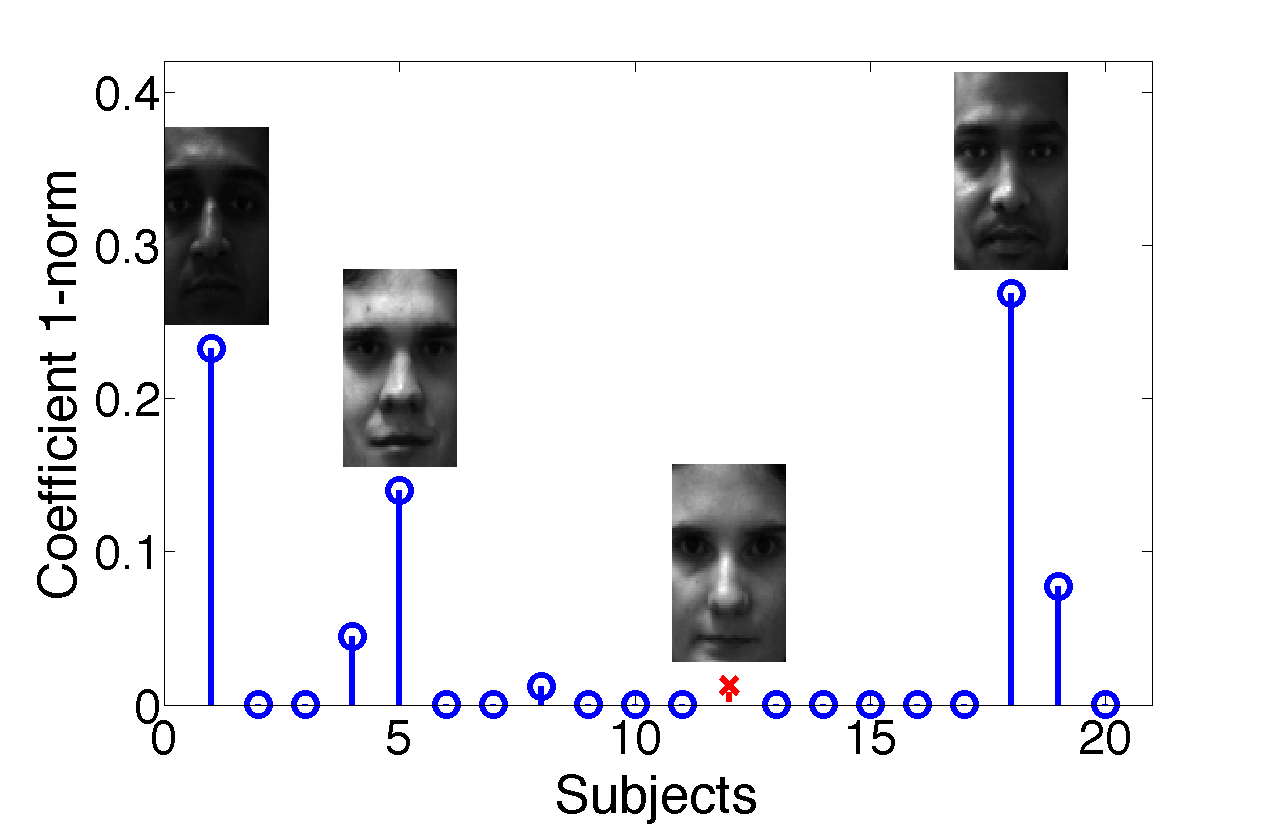
\includegraphics[height=\tempheight]{figures_pami/promo/case2/sci_with_axis_face_case2.png}
\\ 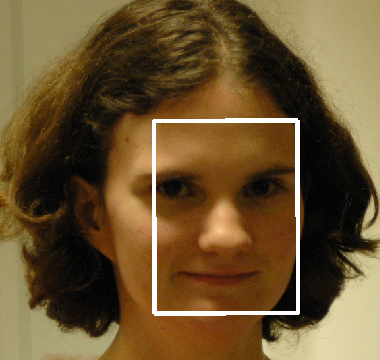
\includegraphics[height=\tempheight]{figures_pami/promo/case3/alignment.png} &
\hspace{3mm}
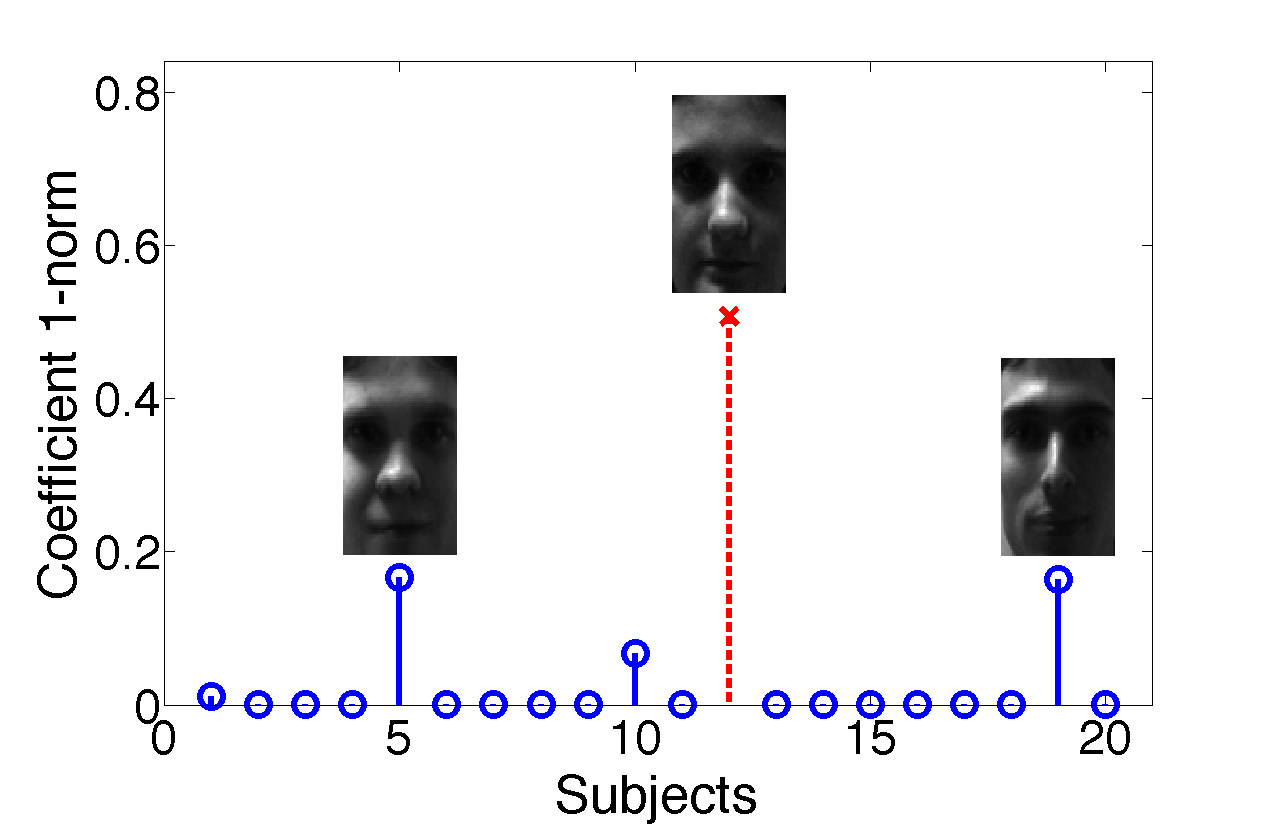
\includegraphics[height=\tempheight]{figures_pami/promo/case3/sci_with_axis_face_case3.png}
\end{tabular} \caption{\small{\bf Effects of registration and illumination on
Recognition}. In this example we identify the girl among 20 subjects by
computing the sparse representation of her input face with respect to the
entire training set. The absolute sum of the coefficients associated with each
subject is plotted on the right. The weighted sum of the 
subject's training images using the associated sparse coefficients is also shown.
The red line (cross) corresponds to her true identity, subject 12. {\bf Top:} The
input face is from Viola and Jones' face detector (the black box) and all 38
illuminations specified in Section \ref{sec:illumination} are used in the
training.  {\bf Middle:} The input face is well-aligned (the white box) with
the training by our algorithm specified in Section \ref{sec:registration}, but
only 24 frontal illuminations are used in the training for recognition (see
Section \ref{sec:illumination}). {\bf Bottom:} The input face is well aligned and
a sufficient set (all 38) of
illuminations are used in the training. Both are necessary for correct recognition
using SRC.}\label{fig:promo}
\end{figure}

\subsection{Relation to Earlier Work on Image Registration}

In holistic recognition algorithms (algorithms that use images themselves as
features) correspondence between points in the test image and in the gallery
images must be achieved.  A long line of research exists on using Active
Appearance Models \cite{Cootes2001-PAMI}, and the closely related Active Shape
Models \cite{cootes1992active} to register images against a relatively
high-dimensional model of plausible face appearances, often leveraging
face-specific contours.  While these model-based techniques have advantages in
dealing with variations in expression and pose, they may add unnecessary
complexity to applications where subjects normally present a neutral face or
only have moderate expression. Instead, this work focuses on classes of
deformations with far fewer degrees of freedom, i.e. similarity transformations
or perspective transformations.  Iterative registration in the spirit of this
work dates at least back to the Lucas-Kanade algorithm
\cite{lucas1981iterative}.

Whereas much of the early work on image registration is aimed at the problem of
registering nearly identical images, say by minimizing a sum of squared
distances or maximizing normalized correlation, face recognition applications
must confront several physical factors simultaneously: misalignment,
illumination variations, and corrupted pixels.  As will be discussed further
below, illumination variation can be dealt with by expressing the test image as
a linear combination of an appropriate set of training images. Similar
representations have been exploited in illumination-robust tracking (e.g.
\cite{Belhumeur1999-PAA,Murase1995-IJCV}).  For robustness to gross errors, the
$\ell_1$-norm of the residual is a more appropriate objective function than the
classical $\ell_2$-norm. Its use here is loosely motivated by theoretical
results due to Cand\`{e}s and Tao \cite{CandesE2005-IT} (see also
\cite{Wright2008-IT}). These two observations motivate the reformulation of the
registration problem as the search for a set of transformations and
illumination coefficients that minimize the $\ell_1$-norm of the representation
error.  The proposed alignment system uses a generalized Gauss-Newton method
which solves a sequence of affine-constrained $\ell_1$-minimization
problems \cite{Osborne1990-JAMSSB,Jittorntrum1980-NM}. Each of these problems
can also be solved efficiently using recently developed first-order techniques
for $\ell_1$-minimization, which are reviewed in \cite{YangA2010-pp}.

% Illumination
Researchers have tried various techniques to deal with illumination variation.
In almost all recognition algorithms where only a single gallery image is
available per individual, illumination effects are regarded as a nuisance that
must be removed before the algorithm can continue.  This is typically done by
making statistical assumptions about how illumination affects the image, and
using those assumptions to extract a new representation that is claimed to be
illumination invariant.  Recent examples include \cite{chen2006total} and
\cite{zhou2007appearance}.  Despite these efforts, truly
illumination-invariant features remain difficult to obtain from a single input
image.  Clearly, if one has the luxury of designing the acquisition system
and the application demands a high recognition rate,
it is then unwise to limit the gallery to a
single image per person.  The proposed recognition system therefore takes the strategy of sampling many
gallery images of each individual under varying illuminations.  These images
are used as the basis for either a convex cone model
\cite{Georghiades2001-PAMI,belhumeur1998set}, or a subspace model
\cite{Basri2003-PAMI}.  Images are captured using a simple-to-construct
projector based light stage.  While similar systems have been used for
other applications, to our knowledge, this
system is the first to use projectors to indirectly illuminate a subject's face for
the purpose of face recognition.

\subsection{Contributions} This chapter demonstrates how registration and
illumination can be simultaneously addressed within a robust sparse
representation framework. Face registration, despite being a challenging
nonlinear problem, can be solved by a series of linear programs that
iteratively minimize the sparsity of the registration error. This leads to an
efficient and effective alignment algorithm for face images that works for a
large range of variation in translation, rotation, and scale, even when the
face is only partially visible due to eyeglasses, closed eyes and open mouth,
sensor saturation, etc.  A sufficient set of training illuminations that is
capable of linearly representing typical indoor and outdoor lighting is
determined empirically, and a practical hardware system based on synchronized
cameras and projectors is developed for capturing them.

The chapter then demonstrates the effectiveness of the proposed new
methods with a complete face recognition system that is {\em
simple, stable, and scalable}. The proposed system performs
robust automatic recognition of subjects from loosely
controlled probe images taken both indoors and outdoors,
using a gallery of
frontal views of the subjects' faces under the proposed
illuminations. An off-the-shelf face
detector\footnote{The OpenCV
implementation of Viola and Jones' face detector
\cite{Viola2004-IJCV} used in this work has become a de-facto standard
within the computer vision research community.} is used to detect faces in the test images.

Extensive experiments are conducted on the proposed system with
both public databases and a face database that is collected by
the proposed acquisition system. The experimental results on
large-scale public face databases show that the algorithm
indeed achieves very good performance on these databases,
exceeding or competing with the state-of-the-art algorithms.
Additionally, the experimental results on the private database
clearly demonstrate that the recognition system not only works well with
images taken under controlled laboratory conditions, but is
capable of handling practical indoor and outdoor illuminations as well.

\noindent{\em Organization of this chapter:} Section \ref{sec:registration}
presents a derivation of the robust registration and recognition algorithm within the sparse
representation framework. It further elaborates on algorithmic implementation issues,
conducts region of attraction experiments with respect to both 2D in-plane
deformation and 3D pose variation, and discusses its relationship to existing
work. Section \ref{sec:illumination} is dedicated to the training acquisition
system. This system is used to investigate empirically how many training
illuminations are required to handle practical illumination variations, and to
suggest a sufficient set of 38 training illuminations. Extensive experiments on
a large-scale public database and on a newly gathered database are conducted in Section
\ref{sec:multipie} and Section \ref{sec:own-data}, respectively, to verify the
proposed system. 

\section{Robust Alignment}\label{sec:registration} As demonstrated in Figure
\ref{fig:promo}(top), the main limitation of the {\em Sparse Representation and
Classification} (SRC) algorithm of \cite{Wright2009-PAMI} is the assumption of
pixel-accurate alignment between the test image and the training set. This
leads to brittleness under pose and misalignment, making it inappropriate for
deployment outside a laboratory setting. The goal of this section is to show
how this weakness can be rectified while still preserving the conceptual
simplicity and good recognition performance of SRC.

SRC assumes access to a database of multiple registered
training images per subject, taken under varying illuminations.
The images of subject $i$, stacked as vectors, form a matrix
$A_i \in \Re^{m \times n_i}$. Taken together, all of the images
form a large matrix $A = [ A_1 \mid A_2 \mid \dots \mid A_K ]
\in \Re^{m \times n}$. As argued in \cite{Wright2009-PAMI}, a
well-aligned test image $\bb_0$ can be represented as a sparse
linear combination $A \x_0$ of all of the images in the
database,\footnote{This assumes that the training illuminations are sufficient. The next section will address how to ensure illumination
sufficiency.} plus a sparse error $\e_0$
due to corrupted pixels. The sparse representation can be recovered by
minimizing the $\ell_1$-norm\footnote{The $\ell_1$-norm of a
vector, denoted by $\|\cdot\|_1$, is the sum of absolute values of its entries.} of
$\x$ and $\e$:
\begin{equation}
\min_{\x,\e} \, \| \x \|_1 + \| \e\|_1 \quad \subj \quad \bb_0 = A \x + \e.
\label{eqn:robust-l1}
\end{equation}
Now suppose that $\bb_0$ is subject to some pose or
misalignment, so that instead of recording $\bb_0$, the camera captures
a warped image $\bb = \bb_0 \circ \tau^{-1}$, for some
transformation $\tau \in T$ where $T$ is a finite-dimensional
group of transformations acting on the image domain.  The
transformed image $\bb$ no longer has a sparse representation of
the form $\bb = A \x_0 + \e_0$, and naively applying the
algorithm of \cite{Wright2009-PAMI} is no longer appropriate,
as seen in Figure \ref{fig:promo}(top).

\subsection{Batch and Individual Alignment} If the
true deformation $\tau^{-1}$ can be found, then
its inverse $\tau$ can be applied to the test image and it again becomes
possible to find a sparse representation of the resulting
image, as $\bb \circ \tau = A \x_0 + \e_0$.\footnote{In the terminology of \cite{baker2004lucas}, this formulation is ``forward additive.''}
  This sparsity
provides a strong cue for finding the correct deformation
$\tau$: conceptually, one would like to seek a transformation
$\tau$ that allows the sparsest representation, via
\begin{equation} \label{eqn:L1-L1-conceptual}
\hat{\tau} = \arg\hspace{-2.5mm}\min_{\x,\e,\tau \in T} \| \x \|_1 + \| \e \|_1 \quad \subj \quad \bb \circ \tau = A \x + \e.
\end{equation}
For fixed $\tau$, this problem is jointly convex in $\x$ and
$\e$. However, as a simultaneous optimization over the
coefficients $\x$, error representation $\e$, and
transformation $\tau$, it is a difficult, non-convex
optimization problem. One source of difficulty is the presence
of multiple faces in the matrix $A$:
\eqref{eqn:L1-L1-conceptual} has many local minima that
correspond to aligning $\bb$ to different subjects. In this
sense, the misaligned recognition problem differs from the
well-aligned version studied in \cite{Wright2009-PAMI}. For the
well-aligned case, it is possible to directly solve for a
global representation, with no concern for local minima. With
possible misalignment, it is more appropriate to seek the best
alignment of the test face with each subject $i$:
\begin{equation} \label{eqn:per-subject-L1}
\hat \tau_i = \arg\hspace{-2.5mm}\min_{\x,\e,\tau_i \in T} \| \e \|_1 \quad \subj \quad \bb \circ \tau_i = A_i \x + \e.
\end{equation}
It no longer makes sense to penalize $\| \x \|_1$, since $A_i$ consists of
only images of subject $i$ and therefore $\x$ is no longer expected to
be sparse.

\subsection{Alignment via Sequential $\ell_1$-Minimization} While the problem
\eqref{eqn:per-subject-L1} is still non-convex, for cases of practical interest
in face recognition, a good initial guess for the transformation is available,
e.g., from the output of a face detector. This initialization can be refined to
approach an estimate of the true transformation by repeatedly linearizing about  the
current estimate of $\tau$, and seeking representations of the form:
\begin{equation}
\bb\circ \tau + J \Delta \tau = A_i \x + \e.
\end{equation}
Here, $J = \frac{\partial}{\partial \tau} \bb \circ \tau$ is the Jacobian of $\bb
\circ \tau$ with respect to the transformation parameters $\tau$, and $\Delta
\tau$ is the step in $\tau$. The above equation is under-determined if the
registration error $\e$ is allowed to be arbitrary. At the correct alignment it
is expected that the test image differs from $A_i \x$ only for the
minority of the pixels corrupted by occlusions. Thus, the algorithm computes a
deformation step $\Delta \tau$ that best sparsifies the registration error
$\e$, in terms of its $\ell_1$-norm:
\begin{equation}
\Delta\hat{\tau}_1 = \arg\hspace{-3.5mm}\min_{\x,\e,\Delta\tau \in T} \| \e \|_1 \quad \subj \quad \bb\circ\tau + J \Delta \tau = A_i \x + \e.
\label{eqn:L1-align}
\end{equation}
This is different from the popular choice that
minimizes the $\ell_2$-norm of the registration error:
\begin{equation}
\Delta\hat{\tau}_2 = \arg\hspace{-3.5mm}\min_{\x,\e,\Delta\tau \in T} \| \e \|_2 \quad \subj \quad \bb\circ\tau + J \Delta \tau = A_i \x + \e,
\label{eqn:L2-align}
\end{equation}
which is also equivalent to finding the deformation step
$\Delta  \tau$ by solving the least-square problem:
$\min_{\x,\Delta \tau} \|\bb \circ \tau + J\Delta \tau - A_i \x
\|_2$. Empirically, if there is only small noise
between $\bb_0$ and $A_i\x$, both \eqref{eqn:L1-align} and
$\eqref{eqn:L2-align}$ have similar performance.  However, if
there are occlusions in $\bb_0$, sequential
$\ell_1$-minimization \eqref{eqn:L1-align} is significantly
better than sequential $\ell_2$-minimization
\eqref{eqn:L2-align}. Figure \ref{fig:L1-L2-align} shows an
example.

The scheme \eqref{eqn:L1-align} can be viewed as a generalized Gauss-Newton
method for minimizing the composition of a non-smooth objective function (the
$\ell_1$-norm) with a differentiable mapping from transformation parameters to
transformed images. Such algorithms date at least back to the 1970s
\cite{Cromme1978-NM,Jittorntrum1980-NM}, and continue to attract attention
today \cite{Lewis2008-TR}. While a detailed discussion of their properties is
outside the scope of this thesis, it is worth mentioning that the scheme
\eqref{eqn:L1-align} is known to converge quadratically in the neighborhood of
any local optimum of the $\ell_1$-norm. In practice, this means that $\approx$
10 to 15 iterations suffice to reach the desired solution. The
interested reader is referred to \cite{Jittorntrum1980-NM,Osborne1990-JAMSSB} and the
references therein.

\renewcommand{\tempheight}[0]{1.0in}
\begin{figure}
\centering
{
\begin{tabular}{cccc}
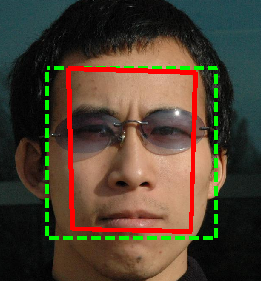
\includegraphics[height=\tempheight]{figures_pami/L1_cropped} &

\includegraphics[height=\tempheight]{figures_pami/y_warp_L1} &

\includegraphics[height=\tempheight]{figures_pami/y_hat_L1} &

\includegraphics[height=\tempheight]{figures_pami/e_L1} \\
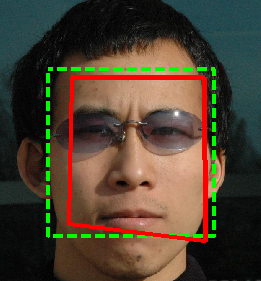
\includegraphics[height=\tempheight]{figures_pami/L2_cropped} &

\includegraphics[height=\tempheight]{figures_pami/y_warp_L2} &

\includegraphics[height=\tempheight]{figures_pami/y_hat_L2} &

\includegraphics[height=\tempheight]{figures_pami/e_L2} \\
(a) & (b) & (c) & (d)
\end{tabular}}
\caption{\small{\bf Comparing alignment of a subject wearing sunglasses by
$\ell_1$ and $\ell_2$-minimization.}
{\bf Top row:} Alignment result of minimizing $\|\e\|_1$. {\bf Bottom row:}
Result of minimizing $\|\e\|_2$. (a) {\em Green (dotted):} Initial face boundary
given by the face detector, {\em Red (solid):} Alignment result shown on the same
face; (b) warped testing image using the estimated transformation $\bb_0$;
(c) reconstructed face $A_i\x$ using the training; (d) image of error $\e$. }\label{fig:L1-L2-align}
\end{figure}

In addition to normalizing the training images (which is done
once), it is important to normalize the warped testing image
$\bb \circ \tau$ as the algorithm runs.  Without normalization,
the algorithm may fall into a degenerate global minimum
corresponding to zooming in on a dark region of the test
image.  Normalization is done by replacing the linearization of
$\bb \circ \tau$ with a linearization of the normalized version
$\tilde \bb(\tau) = \frac{\bb \circ \tau}{\|\bb \circ \tau\|_2}$.
The proposed alignment algorithm can be easily extended to work
in a {\em multiscale} fashion, with benefits both in
convergence behavior and computational cost.  The alignment
algorithm is simply run to completion on progressively less
downsampled versions of the training and testing images, using
the result of one level to initialize the next.

\subsection{Robust Recognition by Sparse Representation} Once
the best transformation $\tau_i$ has been computed for each
subject $i$, the training sets $A_i$ can be aligned to $\bb$,
and a global sparse representation problem of the form
\eqref{eqn:robust-l1} can be solved to obtain a discriminative
representation in terms of the entire training set. Moreover,
the per-subject alignment residuals $\| \e \|_1$ can be used to
prune unpromising candidates from the global optimization,
leaving a much smaller and more efficiently solvable problem.
The complete optimization procedure is summarized as Algorithm
\ref{alg:deformable-src}. The parameter $S$ is the number of subjects
considered together to provide a sparse representation for the
test image. If $S = 1$, the algorithm reduces to classification
by registration error; but considering the test image might be
an invalid subject, $S=10$ is typically chosen. Since valid
images have a sparse representation in terms of this larger
set, invalid test images can be rejected using the {\em sparsity
concentration index} proposed in \cite{Wright2009-PAMI}.
The function $\delta_i(\x)$ in Algorithm \ref{alg:deformable-src}
selects coefficients from the vector $\x$ corresponding to subject $i$.

Another important free parameter in Algorithm \ref{alg:deformable-src} is the
class of deformations $T$. In the experiments presented here, 2D similarity
(i.e. 2D rigid transformations) transformations are used, $T =
\mathbb{SE}(2)\times \Re_+$,\footnote{Here, SE stands for special Euclidean.
The $\Re_+$ accounts for the scale.} for removing alignment error incurred by
face detector, or 2D projective transformations, $T =
\mathbb{GL}(3),\footnote{Here, GL stands for general linear.  This class of
transformations is able to represent distortion in a perspective image of a
planar object.}$ for handling some pose variation.

Algorithm \ref{alg:deformable-src} also implements a simple heuristic
motivated by the observation that the face detector output may be poorly
centered on the face and may contain a significant amount of the background:
before the recognition stage, instead of aligning the training sets to the
original $\bb$ directly obtained from the face detector, the transformations of
the top $S$ classes $\tau_{k_1}, \tau_{k_2}, \ldots, \tau_{k_S}$ are averaged
into a transformation $\bar{\tau}$.  Updating $\bb$ according to $\bar{\tau}$
results in a better centered test image. For the 2D similarity transformations,
which are used in our system when initialized by the face detector, a
transformation $\tau$ can be parameterized as $\tau = (\tau^1, \tau^2, \tau^3,
\tau^4)$, where $\tau^1$ and $\tau^2$ represent the translations in $x$- and
$y$-axis, $\tau^3$ represents the rotation angle and $\tau^4$ represents the
scale. The average transformation is simply obtained by taking the
component-wise mean:
\begin{displaymath}
\bar{\tau}^i = (\tau_{k_1}^i + \tau_{k_2}^i + \cdots +
\tau_{k_S}^i) / S, i = 1,2,3,4.
\end{displaymath}
Finally, the training sets are aligned to the new $\bb$.

\begin{algorithm}[thb]
\caption{\bf\small (Deformable Sparse Recovery and Classification for
Face Recognition)} \label{alg:deformable-src}
\begin{algorithmic}[1]
\begin{small}
\STATE {\bf Input:} Training images $\{A_i \in \Re^{m\times n_i}\}_{i=1}^K$ for $K$ subjects,  a test image
$\bb\in\Re^m$ and a deformation group $T$.
\STATE
{\bf for} each subject $i$,
\STATE \hspace{3mm} $\tau^{(0)}
\leftarrow I$.
\STATE \hspace{3mm} {\bf while} not converged $(j=1,2,\ldots)$ {\bf do}
\STATE \hspace{6mm}
$\tilde \bb(\tau) \leftarrow \frac{\bb \circ \tau}{\|\bb \circ
\tau\|_2}$; \;\;\; $J \leftarrow  \frac{\partial}{\partial
\tau} \tilde\bb(\tau)  \bigr|_{\tau^{(j)}} $;
%\STATE \hspace{6mm} $(\hat \x, \hat \e, \Delta \tau) \leftarrow \left\{\begin{array}{l} \arg \min_{\x,\e,\Delta \tau} \| \e \|_1 \\  \subj \; \bb + J \Delta \tau = A_k \x + \e \end{array}\right.$
\STATE \hspace{6mm} $ \Delta \tau =  \arg\min \; \| \e \|_1  \;
\subj \; \tilde \bb + J \Delta \tau = A_i \x + \e.$
\STATE
\hspace{6mm} $\tau^{(j+1)} \leftarrow \tau^{(j)} + \Delta
\tau$;
\STATE \hspace{3mm} {\bf end while} \STATE {\bf end} \STATE Keep
the top $S$ candidates $k_1, \ldots, k_S$ with the smallest
residuals $\|\e\|_1$. \STATE Compute an average transformation
$\bar{\tau}$ from $\tau_{k_1}, \tau_{k_2}, \ldots, \tau_{k_S}$.
\STATE Update $\bb \leftarrow \bb \circ \bar{\tau}$ and $\tau_i
\leftarrow \tau_i \cdot \bar{\tau}^{-1}$ for $i = k_1, \dots,
k_S$. \STATE Set $A \leftarrow \big[ A_{k_1} \circ
\tau_{k_1}^{-1} \mid A_{k_2} \circ \tau_{k_2}^{-1} \mid \dots
\mid A_{k_S} \circ \tau_{k_S}^{-1} \big]$. \STATE Solve the
$\ell_1$-minimization problem: \\
\hspace{2em}$\hat{\x} = \arg \min_{\x, \e} \| \x \|_1 + \|\e\|_1 \;\; \subj \;\; \bb = A \x + \e.$
\STATE Compute residuals $r_i(\bb) = \| {\bb} - {A}_i \, \delta_i(\hat{\x}) \|_2$ for $i = k_1, \dots, k_S$.
\STATE {\bf Output:} $\mbox{identity}(\bb) = \arg\min_i r_i(\bb)$.
\end{small}
\end{algorithmic}
\end{algorithm}
%\vspace{-4mm}


The transformation $\tau$ defines a mapping between the coordinates of pixels
in the large original image and a smaller (un)warped image. The pixels of the
small image are stacked into a vector. To prevent aliasing artifacts in the
downsampled image, it is necessary to apply a smoothing filter to the original
image beforehand. For a simple implementation, a rectangular window with
regular sampling can be used, but in general, the small image need not be
regularly sampled in pixel coordinates.  For example, the sample locations
could be arbitrarily selected from within a ``face shaped'' area. The impact of
non-rectangular sampling windows on performance of the algorithm will be
discussed in Section \ref{sec:multipie}.

\subsection{System Implementation}
\label{sec:pipeline_implementation}
The runtime of Algorithm~\ref{alg:deformable-src} is dominated
by the time spent solving two qualitatively similar $\ell_1$-minimization problems.
Custom $\ell_1$-minimization solvers for this purpose based on the
\emph{Augmented Lagrange Multiplier} (ALM) algorithm have been developed.
The ALM algorithm was selected because it strikes the best
balance between speed, accuracy, and scalability.  Several $\ell_1$-minimization
algorithms were tested for the face recognition problem, 
and ALM was found to have the best performance. 
A more in-depth discussion of the solvers will be presented
in Chapter \ref{chap:minimization}.
For a more detailed discussion of competing
approaches, the interested reader is referred to
\cite{YangA2010-pp}.
On a Mac Pro with
two Dual-Core 2.66 GHz Xeon processors and 4 GB memory,
running on a private database containing images size $80\times 60$
pixels from 109 subjects under 38 illuminations,
the C++ implementation of Algorithm~\ref{alg:deformable-src} takes
about 0.60 seconds per subject for alignment and about 2.0
seconds for global recognition. Compared to the highly
customized interior point method first presented in 
\cite{Wagner2009-CVPR}, this new algorithm is
only slightly faster for per subject alignment. However, it is
much simpler to implement and it achieves a
\emph{speedup of more than a factor of 10} for global
recognition!  Performance optimization of this algorithm
will be discussed in Chapter \ref{chap:parallel}.

\subsection{Experiments on Region of Attraction} Three experimental results
will now be presented to demonstrate the effectiveness of the individual
alignment procedure outlined in the previous section. They show sufficiency of
the region of attraction, verify effectiveness of the multiscale extension, and
show stability to small pose variations.  After a discussion of illumination
invariance in the next section, large-scale recognition experiments are
presented in Sections \ref{sec:multipie} and \ref{sec:own-data}.

\noindent {1) \em 2D Deformation.}  The first experiment verifies the
    effectiveness of our alignment algorithm with images
    from the CMU Multi-PIE Database \cite{Gross2008-FGR}.
    The gallery set consists of all the subjects in Session 1, using 7
    illuminations per person. The test images use
    one new illumination from each user in Session
    2.\footnote{The training are illuminations $\{0, 1, 7,
    13, 14, 16, 18\}$ of \cite{Gross2008-FGR}, and the
    testing is the illumination 10. } A ground truth for
	registration is formed by manually selecting
    eye corners in both training and testing images. 
	The images are downsampled to a canonical image size of 
    $80\times 60$ pixels\footnote{Unless otherwise stated,
    this will be the default resolution at which 
    all training and testing data sets are resampled.} 
	and the distance between the two outer
    eye corners is normalized to be 50 pixels for each
    person. An artificial deformation is applied to the
    testing image with a combination of translation,
    rotation and scaling. A small value for the alignment
    error $r = \|\e\|_1$ is chosen as an indicator of success. Let $r_0$
    be the alignment error obtained by aligning a test
    image to the training images without any artificial
    perturbation. After the test image is artificially
    perturbed and aligned resulting in an alignment error
    $r$, we consider the alignment successful if $|r - r_0 | \leq
    0.01r_0$. Figure \ref{fig:attraction} shows the
    percentage of successful registrations for all subjects
    for each artificial deformation. The results suggest
    that the alignment algorithm works extremely well with
    translation up to 20\% of the eye distance (or 10
    pixels) in all directions and up to $30^\circ$ in-plane
    rotation. Tests of the alignment algorithm
    with scale variation show that it can handle up to 15\%
    change in scale.

In order to determine if this region of attraction is sufficient,
it must be compared to the accuracy achieved by the initialization
provided by the face detector.  This is done by gathering statistics 
of the Viola and Jones'
 face detector on the Multi-PIE data set: For 4,600 frontal
 images of 230 subjects under 20 different illuminations,
 using manual registration as the ground truth, the average
 misalignment error of the detected faces is about 6 pixels
 and the average variation in scale is 8\%. This falls
 safely inside the region of attraction of the alignment
 algorithm.
\newcommand{\tempheighta}[0]{1.1in}
\newcommand{\tempheightb}[0]{0.9in}
\begin{figure*}
\centering
{
\begin{tabular}{ccc}
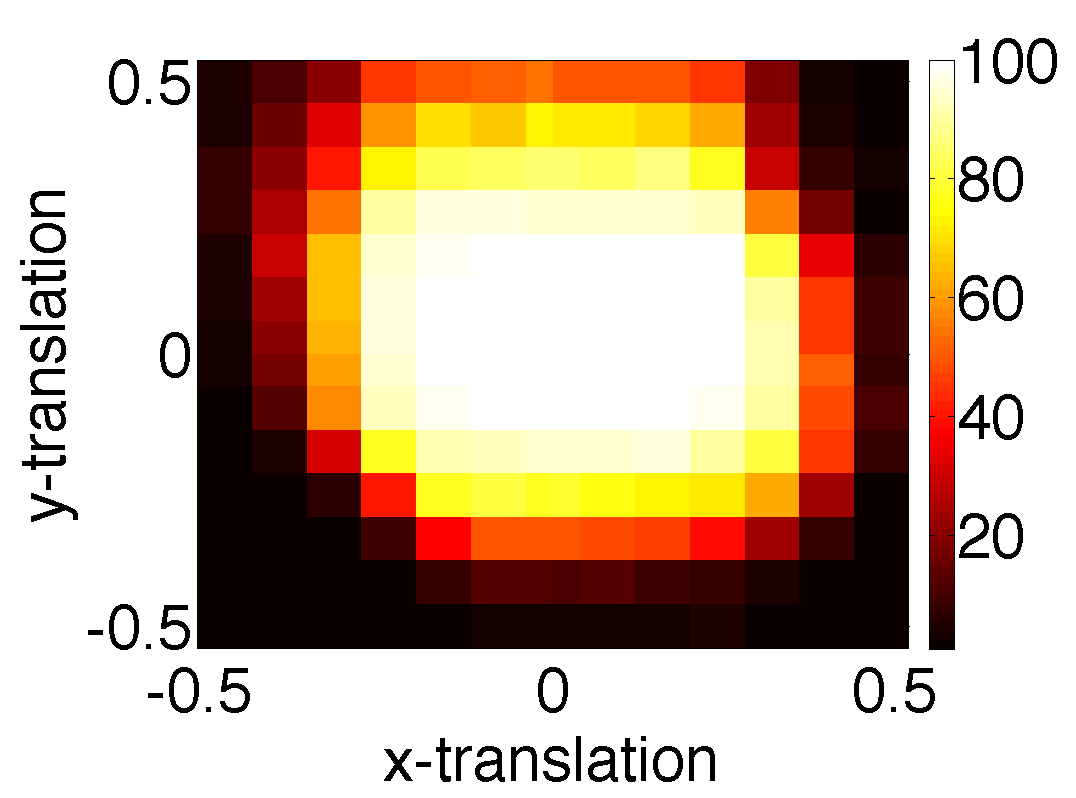
\includegraphics[height=\tempheighta]{figures_pami/x_y_roa.png} &
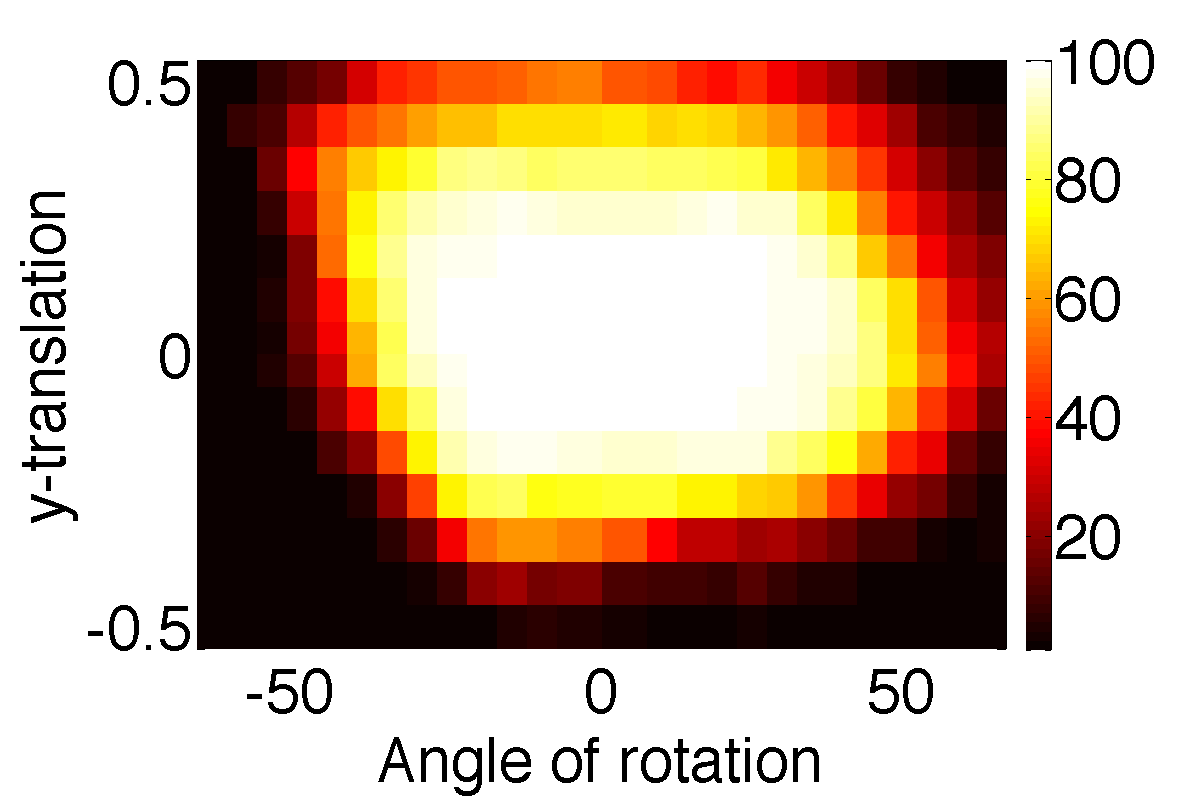
\includegraphics[height=\tempheighta]{figures_pami/y_theta_roa.png} &
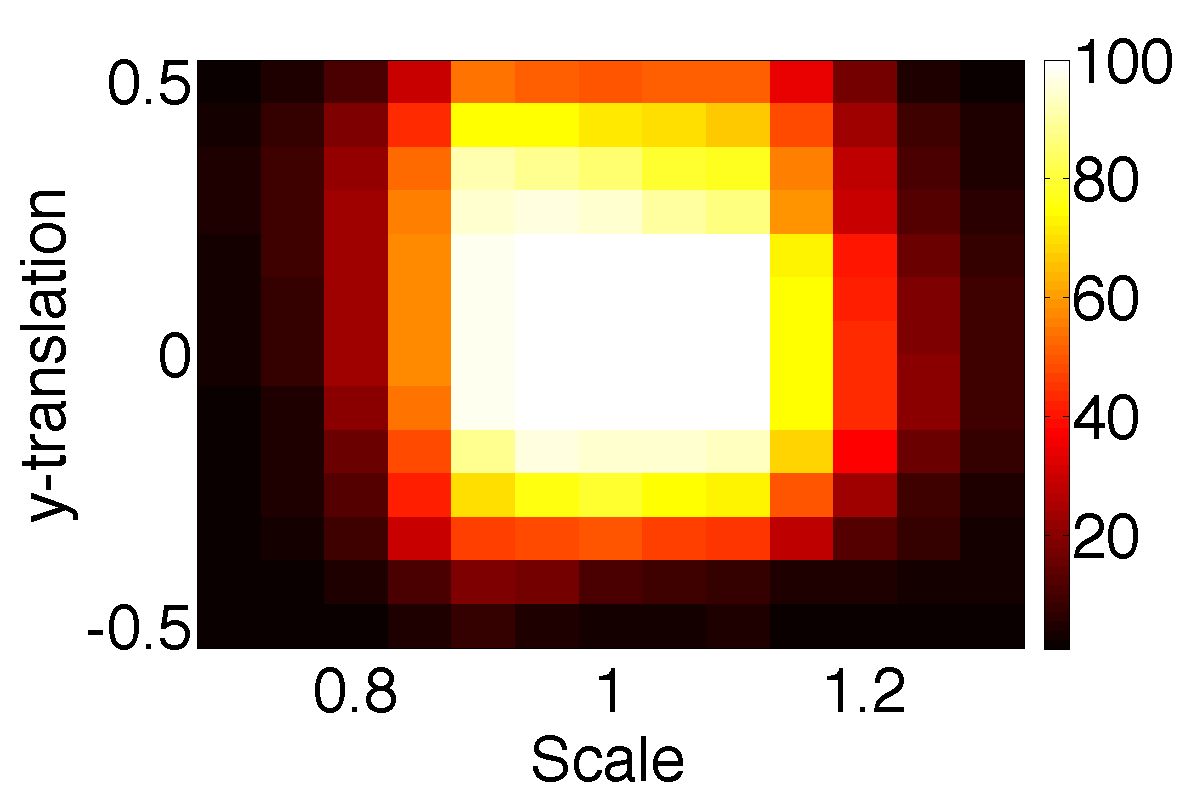
\includegraphics[height=\tempheighta]{figures_pami/y_s_roa.png}\\
(a)&(b)&(c)
\end{tabular}
\begin{tabular}{cccc}
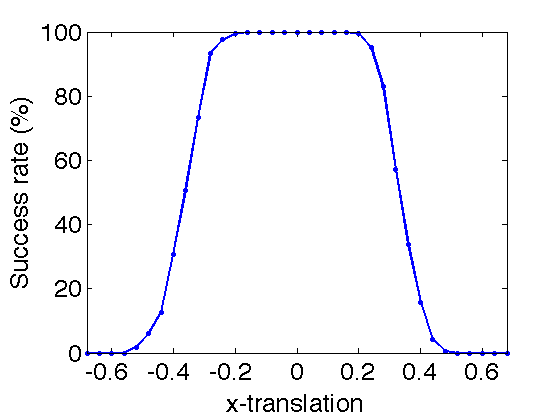
\includegraphics[height=\tempheightb]{figures_pami/x_tr.png} &
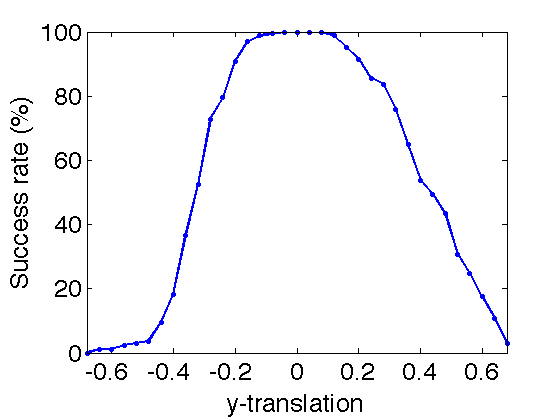
\includegraphics[height=\tempheightb]{figures_pami/y_tr.png} &
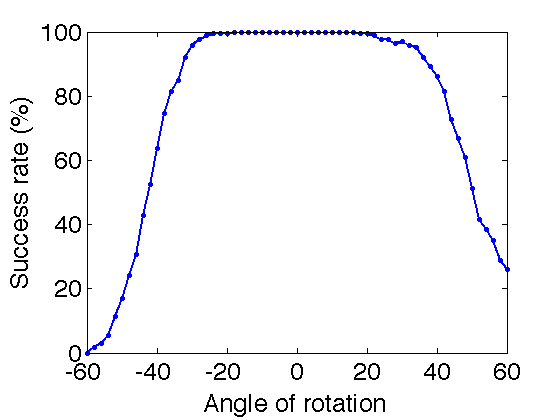
\includegraphics[height=\tempheightb]{figures_pami/theta.png} &
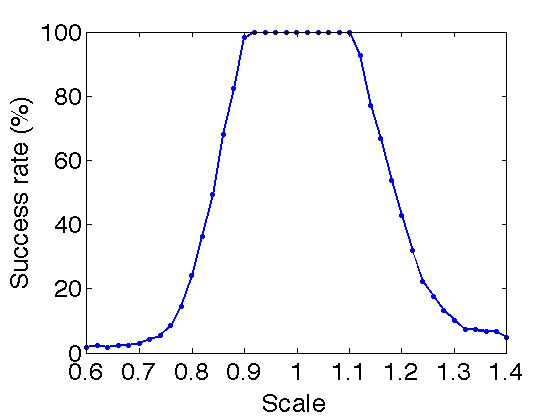
\includegraphics[height=\tempheightb]{figures_pami/scale.png}\\
(d)&(e)&(f)& (g)
\end{tabular}
} \caption{\small{\bf Region of attraction.} Fraction of
subjects for which the algorithm successfully aligns a
synthetically perturbed test image.  The amount of translation
is expressed as a fraction of the distance between the outer
eye corners, and the amount of in-plane rotation in degrees.
{\bf Top row:} (a) Simultaneous translation in $x$ and $y$
directions. (b) Simultaneous translation in $y$ direction and
in-plane rotation. (c) Simultaneous translation in $y$
direction and scale variation. {\bf Bottom row:} (d)
Translation in $x$ direction only. (e) Translation in $y$
direction only. (f) In-plane rotation only. (g) Scale variation
only.} \label{fig:attraction} 
\end{figure*}

\noindent{2) \em Multiscale Implementation.}
Performing alignment in a multiscale fashion has two benefits: first, it
provides a larger region of attraction, and second, it reduces overall
computational cost. This experiment investigates the convergence behavior of
the alignment algorithm as a function of the standard deviation $\sigma$ of the
Gaussian smoothing filter and the number of scales considered.
The experiment is performed using the same 7 illuminations from
Session 1 as training, and all 20 illuminations in the same
session as testing. The images are artificially deformed in
both $x$ and $y$ directions by up to 16 pixels in the
$80\times 60$ frame, with a step size of 4 pixels, i.e.,
$(\Delta x, \Delta y) \in \{-16,-12,\ldots,12,16\} \times
\{-16,-12,\ldots,12,16\}$. An alignment is considered
successful if the estimated coordinates of the eye-corners
are within 1 pixel from the ground truth in the original
image.  Figure \ref{fig:multiscale} shows the
alignment success rate, averaged over the artificially
perturbed initial deformations, as a function of the
standard deviation of the Gaussian kernel $\sigma$, for
three choices of the number of scales. 
Using multiscale indeed improves the performance, and when
3 scales are used, a smaller convolution kernel can achieve
a similar performance compared to a much larger kernel when
only 2 scales are used.
\begin{figure}
\centering
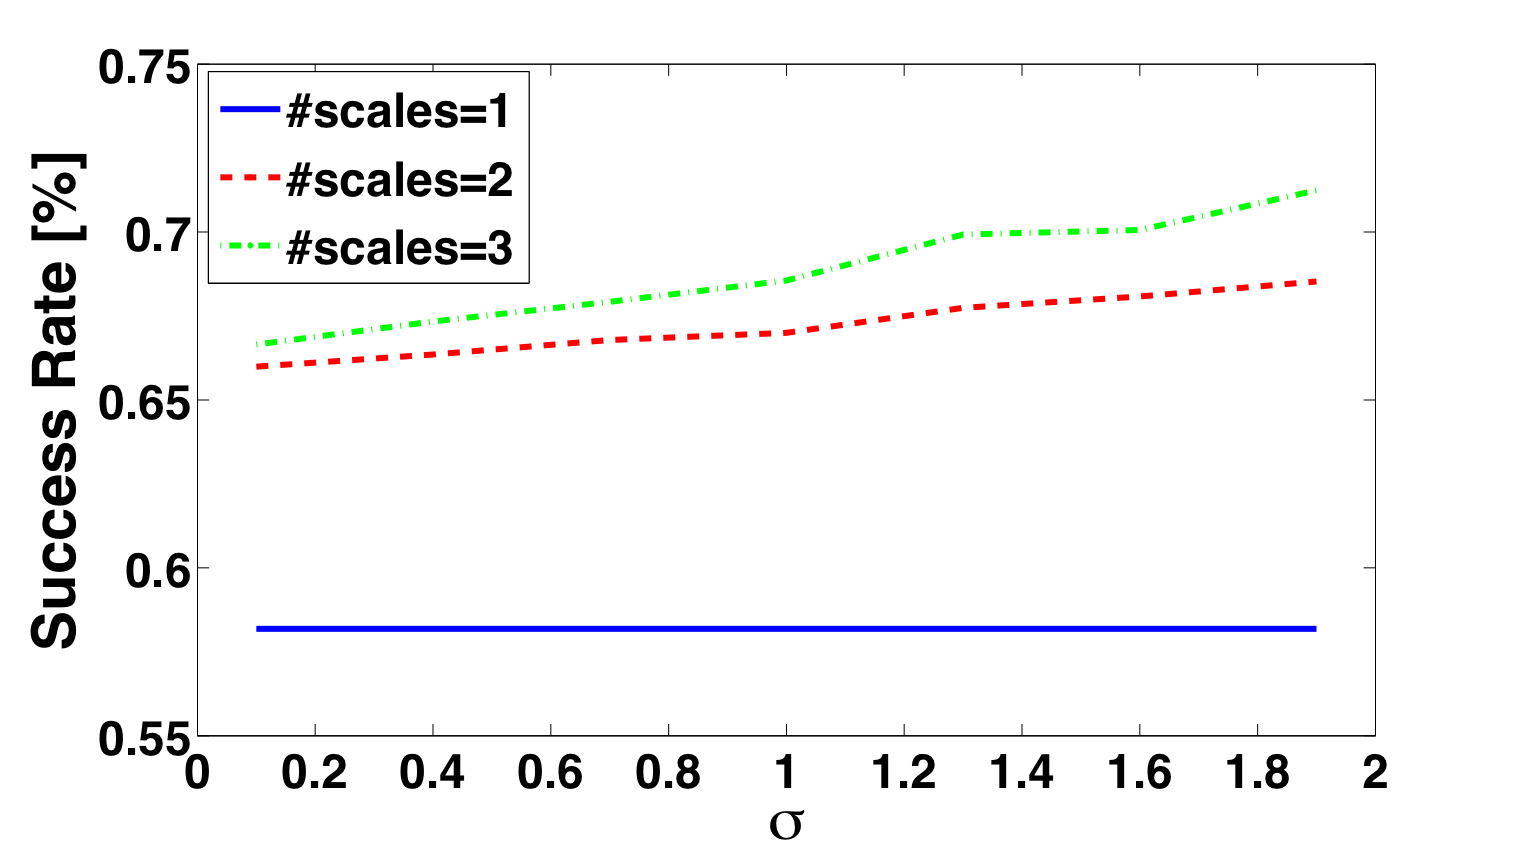
\includegraphics[width=4in]{figures_pami/multiscale.png}
\caption{\small{\bf Multiscale alignment.} This figure shows the average success rate of 
alignment over all possible perturbations. A smaller blur kernel can be applied to achieve 
better performance when more scales are used.}
\label{fig:multiscale}
\end{figure}

\noindent{3) \em 3D Pose Variation.} Since densely sampled pose and
    illumination face images are not available in any of
    the public databases, including Multi-PIE, a private
	data set has been collected using the training image
	acquisition system described in the next section.
	Frontal face images of each subject under the 38 illuminations proposed
    in the next section are used as training images. Test
	images of each subject are collected under typical indoor
    lighting conditions at pose ranging from $-90^\circ$ to
    $+90^\circ$ with step size 5.625$^\circ$, a total of 33
    poses. The alignment algorithm is initialized using 
	Viola and Jones' face detector.
	Figure \ref{fig:pose-alignment} shows that the alignment algorithm 
	appears to achieve reasonable alignments
	with poses up to $\pm 45^\circ$.
Note that this level of out-of-plane
 pose variation is well beyond what the 2D image recognition system
intended to handle, and recognition performance will likely start
to suffer at lower out-of-plane head angles.
\begin{figure}
\centering
{
\begin{tabular}{ccccc}
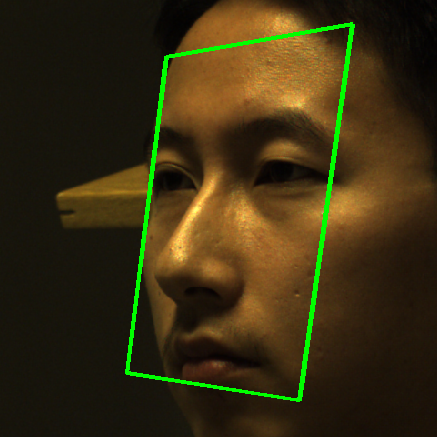
\includegraphics[height=1in]{figures_pami/5} &
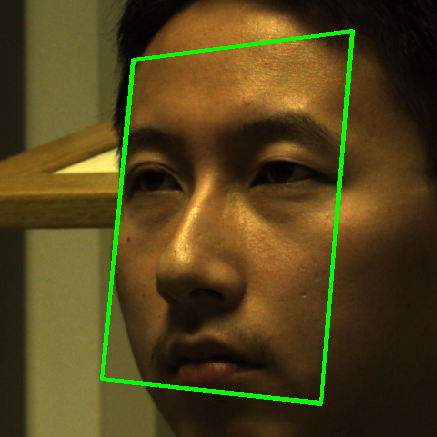
\includegraphics[height=1in]{figures_pami/7} &
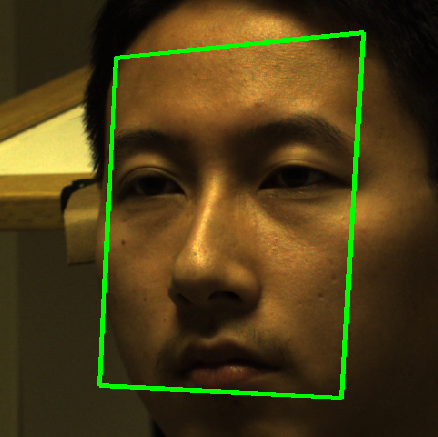
\includegraphics[height=1in]{figures_pami/09} &
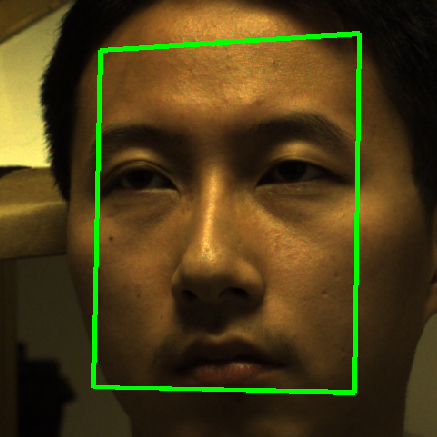
\includegraphics[height=1in]{figures_pami/11} &
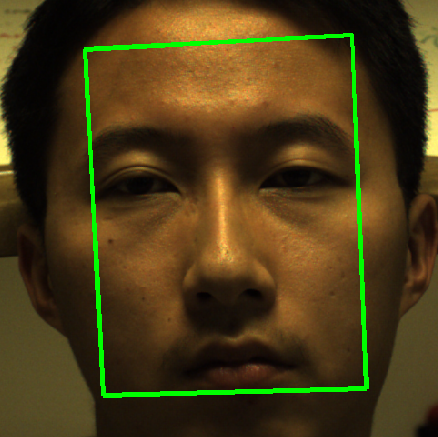
\includegraphics[height=1in]{figures_pami/13} \\
(a) & (b) & (c) & (d) & (e)\\
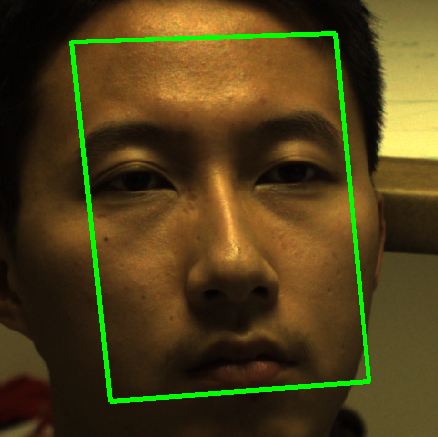
\includegraphics[height=1in]{figures_pami/15} &
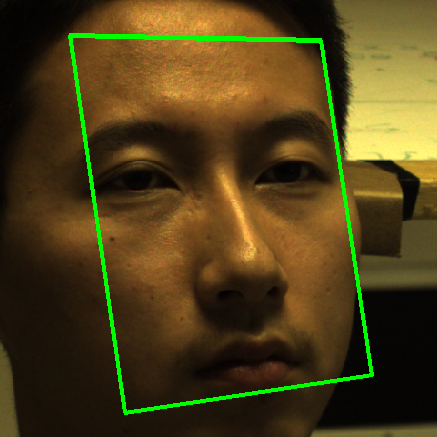
\includegraphics[height=1in]{figures_pami/17} &
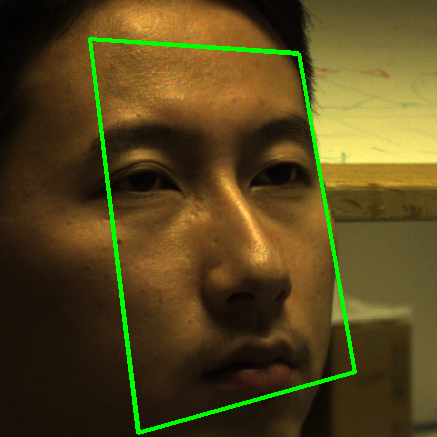
\includegraphics[height=1in]{figures_pami/19} &
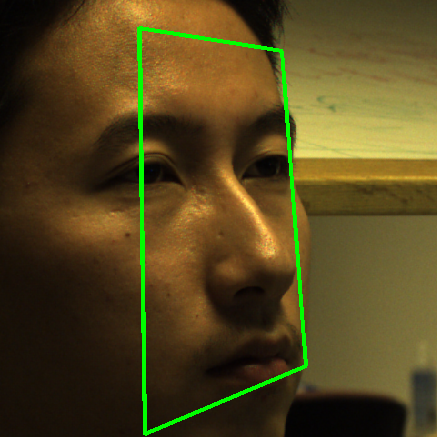
\includegraphics[height=1in]{figures_pami/21} &
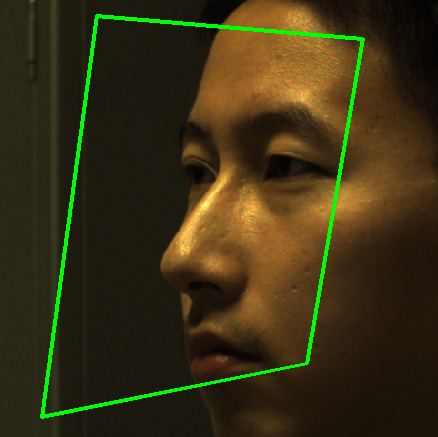
\includegraphics[height=1in]{figures_pami/3} \\
(f) & (g) & (h) & (i) & (j)
\end{tabular}
}
\caption{\small{\bf 2D Alignment of test images with different poses to frontal training images.} {\bf (a) to (i):}  plausible alignment for pose from $-45^{\circ}$
to $+45^{\circ}$. {\bf (j):} a case when the algorithm fails for an extreme pose ($>45^{\circ}$).
}\label{fig:pose-alignment} 
\end{figure}
\subsection{Comparison with Related Work}
The enhancements to SRC presented in this chapter are rooted 
solidly in the tradition of
adding deformation-robustness to face recognition algorithms
\cite{Cootes2001-PAMI,Gross2006-PAMI,Wiskott1997-PAMI}.
However, the only previous work to investigate face alignment
in the context of sparse signal representation and SRC is the
work of \cite{Huang2008-CVPR}. They consider the case where the
training images themselves are misaligned and allow one
deformation per training image. They linearize perturbation of the training
set rather than the test, which is computationally more costly as
it effectively quadruples the size of the training set. 
Additionally, since they align the test image to all subjects
simultaneously, their alignment iteration is likely more prone 
to getting stuck in local minima when there is a large number
of subjects in the gallery.  The effects of this will be seen
in the following experimental comparisons.
\begin{enumerate}
\item {\em Extended Yale B.} In this experiment, the
    same experimental settings are used as in
    \cite{Huang2008-CVPR}. 20 subjects are selected and
    each has 32 frontal images (selected at random) as
    training and another 32 for testing. An artificial
    translation of 10 pixels (in both $x$ and $y$
    directions) is introduced to the test image. For our
    algorithm we downsample all of the images to $88\times
    80$ for memory reasons, whereas the work of
    \cite{Huang2008-CVPR} uses random projections.
	Note that the use of cropped images in this 
	experiment introduces image boundary effects.
    The proposed $\ell_1$-minimization based alignment
    algorithm achieves a recognition rate of 93.7\%,
    compared to a 89.1\% recognition rate reported in
    \cite{Huang2008-CVPR}.
\item {\em CMU Multi-PIE.} This experiment is performed
	using
    all subjects from the CMU Multi-PIE database, 7
    training images from Session 1 and 1 test image from
    Session 2 per person. The setting is exactly the same
    as the previous experiment on 2D deformation. Images are again
    downsampled to a canonical size of $80\times 60$ pixels. An
    artificial translation of 5 pixels (in both $x$ and $y$
    directions) was induced in the test image. The
    algorithm of \cite{Huang2008-CVPR} achieves a
    recognition rate of 67.5\%,\footnote{That algorithm has
    two free parameters - $l$ and $d$, which govern the trade-off between
	accuracy and runtime. For this experiment
    these values are chosen to be $l = 1$ and $d = 514$.} while 
	$\ell_1$-minimization based alignment achieves 92.2\%.
    \end{enumerate}
				
\section{Handling Illumination Variation}
\label{sec:illumination}
In the above section, it was assumed that the test image, although taken under
some arbitrary illumination, can be linearly represented by a finite number of
training illuminations.  Under what conditions is this a reasonable assumption
to make?  What can be said from first principles about how the training images
should be chosen?

\subsection{The Illumination Model}
%
The strongest theoretical results so far regarding the relationship between
illumination and the resulting sets of images is due to Basri and Jacobs
\cite{Basri2003-PAMI}.  The main result is that for convex Lambertian objects,
distant illuminations, and fixed pose, all images of the object can be well
approximated by linear combinations of nine (properly chosen) basis images.
These basis images have mixed sign, and their illuminations consist of the
lowest frequency spherical harmonics.  While this is a very important result
for understanding the image formation process, the direct application of this
result in most practical systems is misguided for several reasons.\footnote{A more
thorough discussion of this result can be found in 
Appendix \ref{chap:appendix_illumination}, and more discussion of linearity can be found in
\cite{belhumeur1998set}.}
Specularities, self-shadowing, and
inter-reflections all dramatically affect the appearance of face images, and
they all do so in a way that violates the modeling assumptions of the Basri
analysis.

Fortunately, even with these effects, for most materials the relationship
between illumination and image is still linear,\footnote{Materials that break
this assumption include fluorescent materials and the photochromic
(``Transition'') lenses in some eyeglasses.  Most materials emit light in
proportion to their incident light.} provided the sensor has a linear response
curve.\footnote{Proper handling of gamma encoding is an important consideration
for practitioners.  Most cameras apply a non-linear and often undocumented
response curve to captured images.  A slight degradation of performance will
occur if gamma compressed images are treated as if they were linear.  The best
performance is achieved either with machine vision cameras with a linear
response curve, or with cameras with calibrated response curves that can be
inverted when the image file is loaded.} While the relationship between
illuminations and images is linear, only positive weights are allowed; the
space of all images of an object with fixed pose and varying illumination is a
convex cone lying in the positive orthant. The question becomes, how many
images does it take to do a good job of representing images sampled from this
cone?

It has been observed in various empirical studies that one can get away with
using a small number of frontal illuminations to linearly represent a wide
range of new frontal illuminations, when they are all taken under the same
laboratory conditions \cite{Georghiades2001-PAMI}. This is the case for many
public face data sets, including AR, ORL, PIE, and Multi-PIE.  Unfortunately, it
has been found that in practice, a training database consisting purely of
frontal illuminations is not sufficient to linearly represent images of faces
taken under typical indoor or outdoor conditions (see the experiment conducted
in Section \ref{sec:own-data}). As illustrated by the example in Figure
\ref{fig:promo}, an insufficient number of training illuminations can result in
recognition failure. To ensure that the proposed recognition pipeline works in
practice, we need to find a set of training illuminations that are indeed {\em
sufficient} to linearly represent a wide variety of practical indoor and
outdoor illuminations.

\subsection{Projector-Based Illumination System}
%
This section describes a novel system that can acquire frontal images of a
subject while simultaneously illuminating the subject from all above-horizontal
illumination directions. A sketch of the system is shown in Figure
\ref{fig:system}: The illumination system consists of four projectors that
display various bright patterns onto the three white walls in the corner of a
dark room.  The light reflects off of the walls and illuminates the user's head
indirectly.  After the frontal illuminations are acquired, the chair is rotated by
180 degrees and a second set of pictures are taken from the opposite direction
so that the subject is illuminated from behind and above.  In practice, having
two cameras greatly accelerates the process since only the chair needs to be
moved in between frontal and rear illuminations. This projector-based system
has several advantages over flash-based illumination systems for face
recognition:
\begin{itemize}
\item The illuminations can be modified in software, rather than hardware.
\item It is easy to capture many different illuminations quickly.
\item Good coverage and distant illumination can be achieved simultaneously.
\item There is no need to mount anything on the walls or construct a large dome.
\item The system can be assembled from off-the-shelf hardware.
\end{itemize}
\begin{figure}
\centering
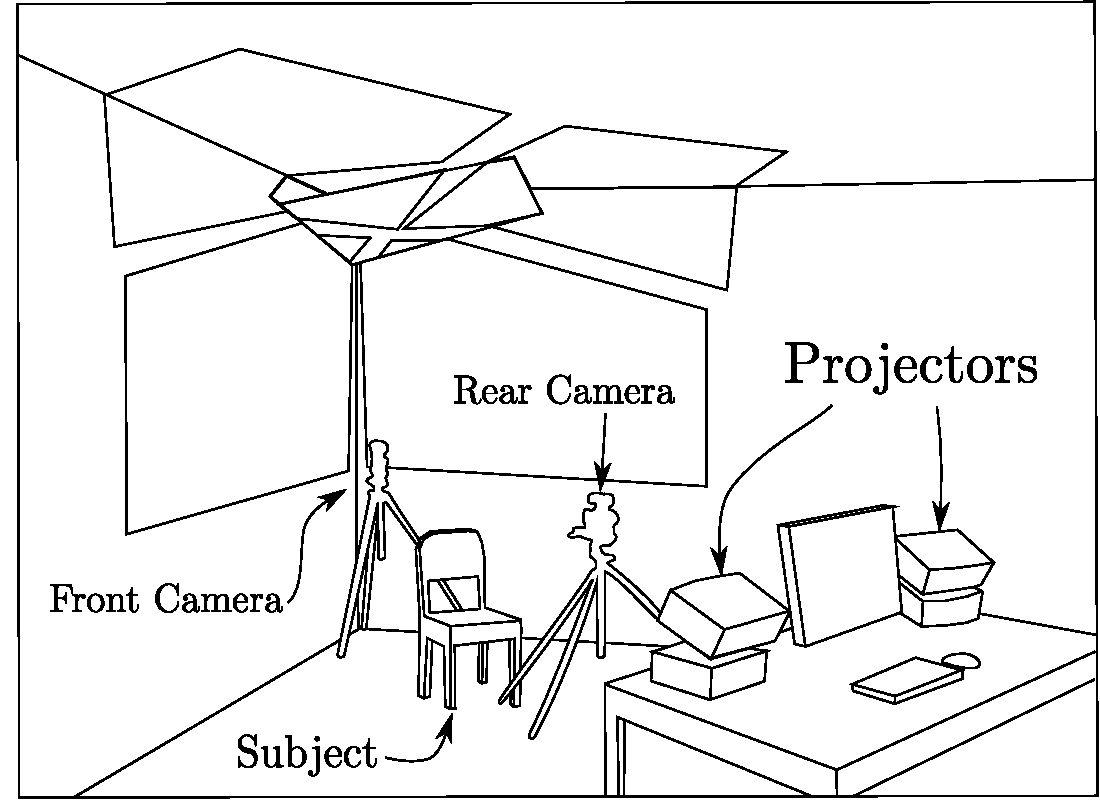
\includegraphics[height=2.5in]{figures_pami/camera_rig.pdf}
\caption{\small{\bf Training acquisition system:} Four projectors and two cameras controlled by one computer.}
\label{fig:system}
\end{figure}
%
With this projector system, the choice of illumination patterns is constrained
only by the need to achieve a good signal-to-noise-ratio (SNR),\footnote{Since
illuminations with more pixels illuminated will have a better SNR (provided
they don't saturate), there is an engineering tradeoff between the SNR and the
number of training images.} avoid saturation, and achieve a reasonably short
acquisition time.  Two simplifying assumptions that we make are that every
pixel is either turned fully on or off in every illumination, and that the
illuminated regions do not overlap.

Assuming that each pixel is fully on or off makes it possible to guarantee that each
illumination image has the same overall intensity, merely by guaranteeing that
the same number of pixels are illuminated in each image.\footnote{Since DLP
projectors may have dramatically different response curves depending on the
mode they are in, it is not advisable to simply normalize each illumination
image by its mean.} Since our algorithm depends only on the linearity between
the illuminations and the images, and not on the relative intensities of the
illuminations, the designer has the freedom to choose the overall intensity of
the illuminations to prevent saturation or low SNR, in a sort of offline
exposure control.

The assumption that the sequentially illuminated regions do not overlap results in a
set of training images that span a larger cone than a similar number of
overlapping regions.  This results in training images that require fewer
negative coefficients in $\x$ to represent test images under natural
illuminations.  The effect of negative coefficients in $\x$ appears to depend
partly on how the test images are taken and is still under study.
This is discussed further in Appendix \ref{chap:appendix_illumination}.

{\em Relationship to existing work:} Most light stages used for face
recognition have been constructed for the purpose of creating public data sets
to study illumination invariance \cite{Georghiades2001-PAMI, Gross2008-FGR}.
Many other light stages have been used for computer graphics purposes
\cite{debevec2000acquiring, jones2005performance}.  The light source can be
moved around manually \cite{masselus2002free}, but this may result in poor
consistency of illuminations between users.  Structured light applications use
projectors to directly illuminate the face (or other object)
\cite{zhang2002rapid} for 3D reconstruction, but this is very disturbing to the
user.  Y.\ Schechner et al.\cite{schechner2007multiplexing} study techniques for
multiplexing illumination that can dramatically reduce the noise of the
demultiplexed images for certain classes of objects and cameras.  While these
techniques have not been incorporated into the current system, they fit
elegantly into the framework and will likely be used in future implementations.
To avoid confusion, it must be emphasized that use of this multiplexing
technique is independent from the choice of original (directional)
illuminations, which is addressed in the next subsection.

\subsection{Choice of Illumination Patterns}

Two experiments are used to motivate the choice of illuminations 
used in the large-scale experiments:
\begin{enumerate}
\item {\em Coverage Experiment.} The first experiment 
    attempts to determine what coverage of the sphere is
    required to achieve good interpolation for test images.
    The subject is illuminated by 100 (50 front, 50 back)
    illuminations arranged in concentric rings centered at
    the front camera.  Subsets of the training images are
    chosen, starting at the front camera and adding a ring
    at a time.  Each time a ring is added to the training
    illumination set, the average $\ell_1$ registration
    error (residual) for a set of test images taken under
    sunlight is computed and plotted in Figure
    \ref{fig:illumination-patterns}(a).  The more rings of
    training illuminations are added, the lower the
    representation error becomes, with diminishing returns.
\item {\em Granularity Experiment.} The second
    experiment attempts to determine how finely divided
    the illumination sphere should be.  At the first
    granularity level, the projectors illuminate the
    covered area uniformly.  At each subsequent granularity
    level, each illuminated cell is divided in two along its
    longer side but its intensity is doubled.  For each
    granularity level the average $\ell_1$ registration
    error is computed as in the coverage experiment and
    shown in Figure \ref{fig:illumination-sufficiency}(b).
    Again, diminishing returns are observed as more
    illuminations are added.
\end{enumerate}
\begin{figure}
\centering
\begin{tabular}{cc}
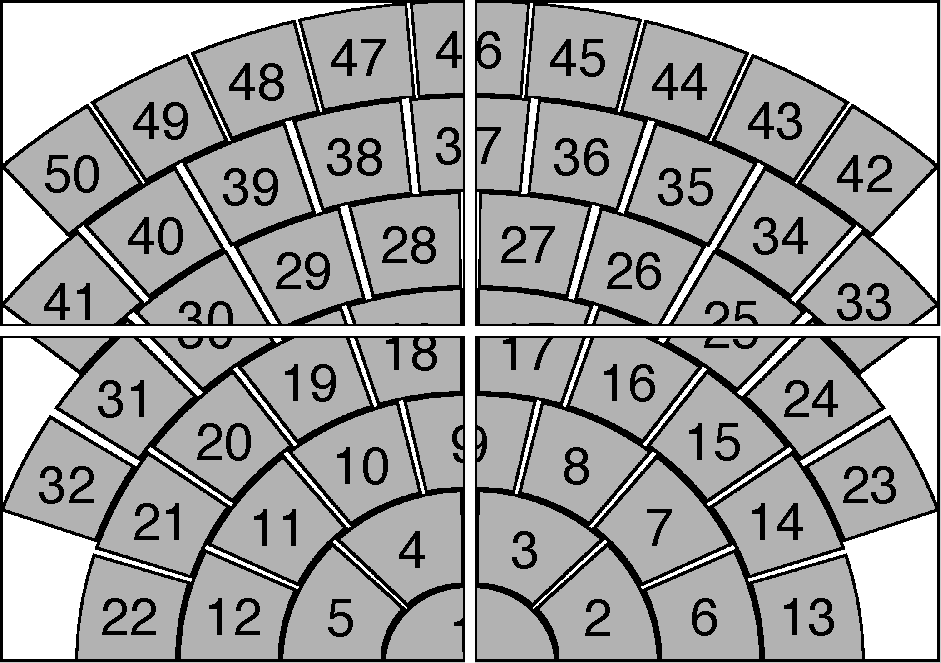
\includegraphics[height=1.7in]{figures_pami/coverage_experiment_asplode.png} &
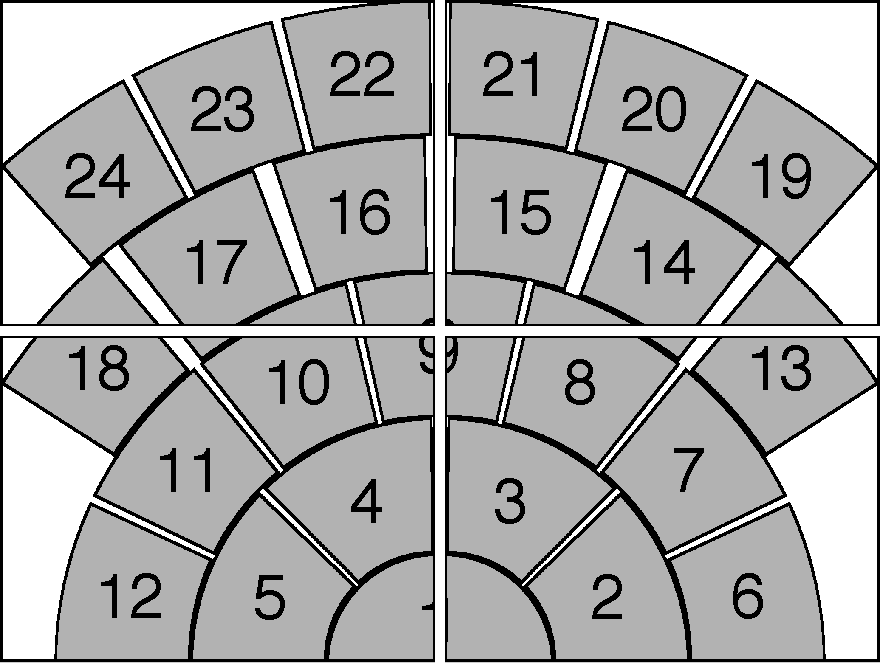
\includegraphics[height=1.7in]{figures_pami/final_cvpr_illuminations_asplode.png}  \\
(a) Coverage Experiment & (b) Chosen Illumination Patterns
\end{tabular}
\caption{\small{\bf Illumination Patterns.}   The cells are illuminated in
sequence.  For rear illuminations the sequence is reversed.  In the chosen
pattern's rear illumination, the cells 1-5 and 7-11 are omitted for a total of
38 illuminations. The four rectangular regions correspond to the four
projectors.  }
\label{fig:illumination-patterns}
\end{figure}

\begin{figure}
\centering
\begin{tabular}{@{}c@{}c@{}}
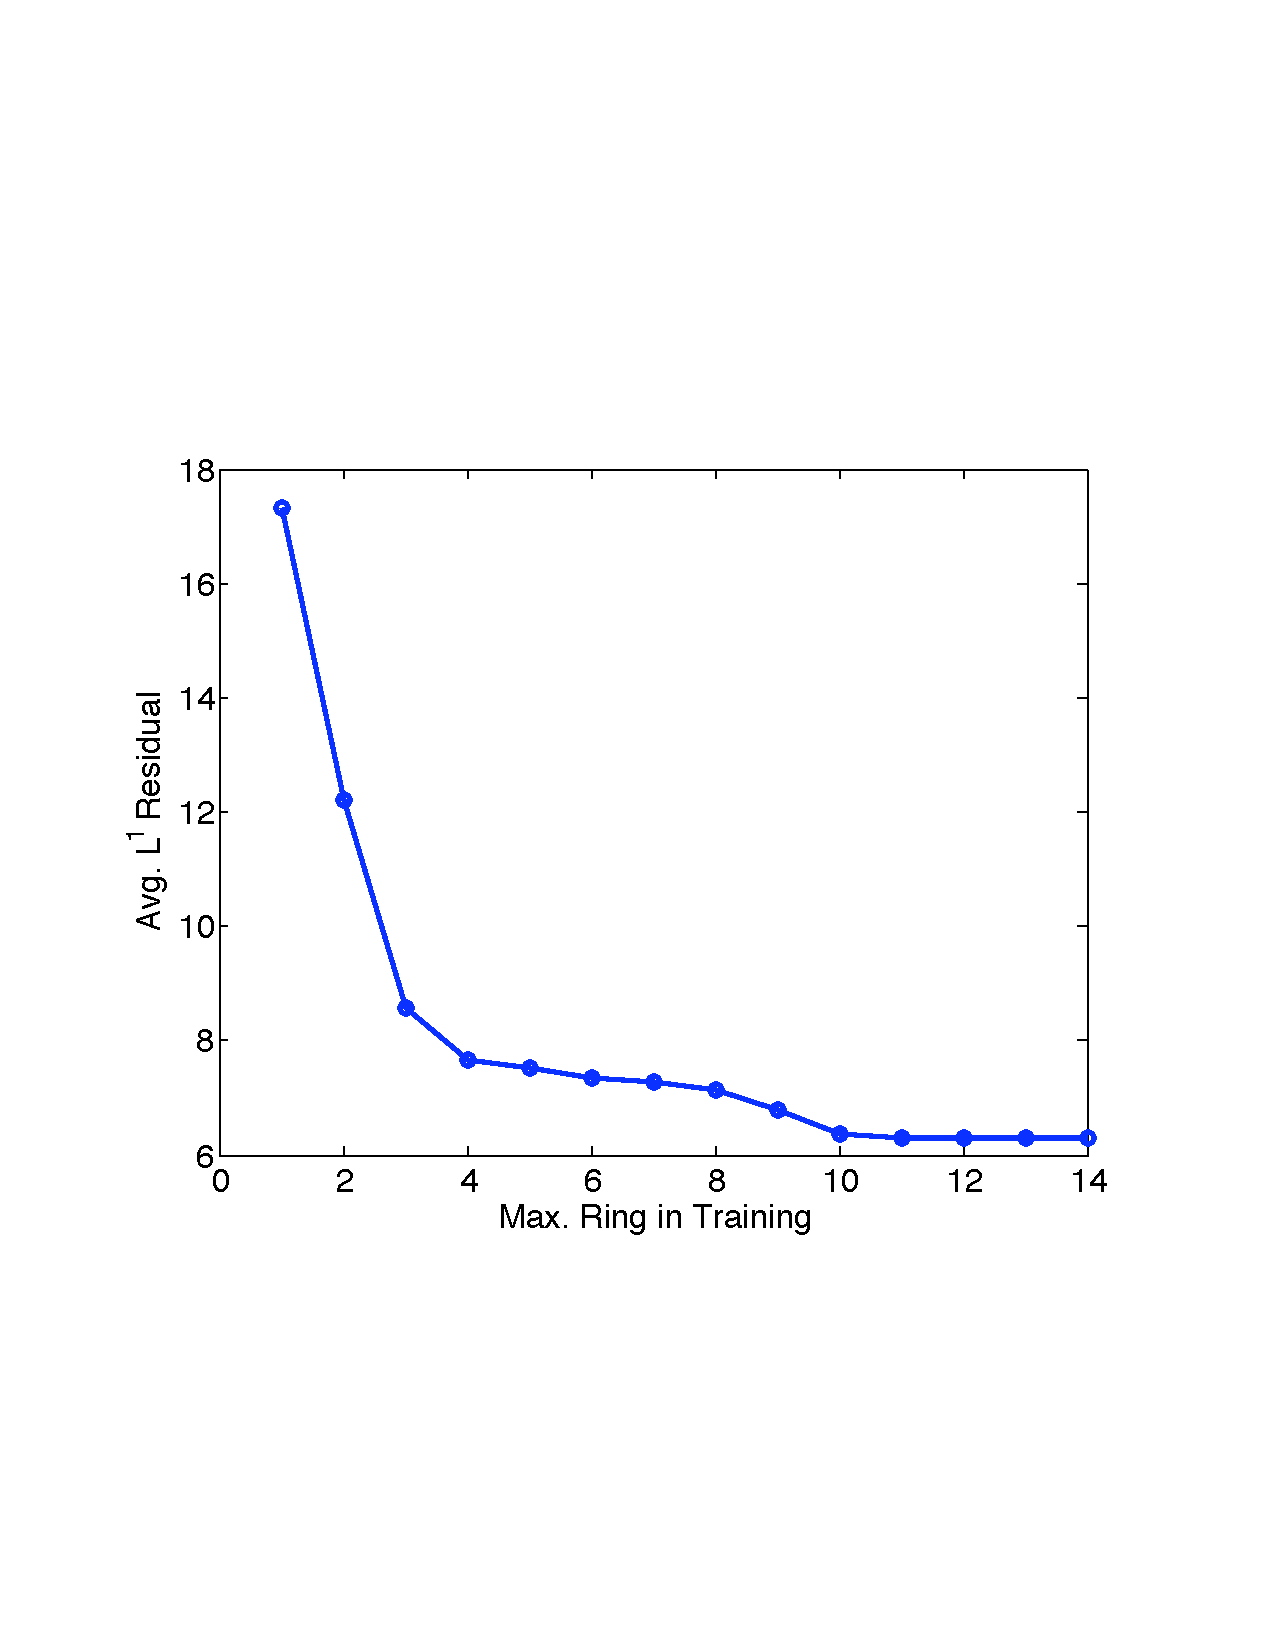
\includegraphics[height=2in]{figures_pami/illum_results/coverage_sunset.pdf} &
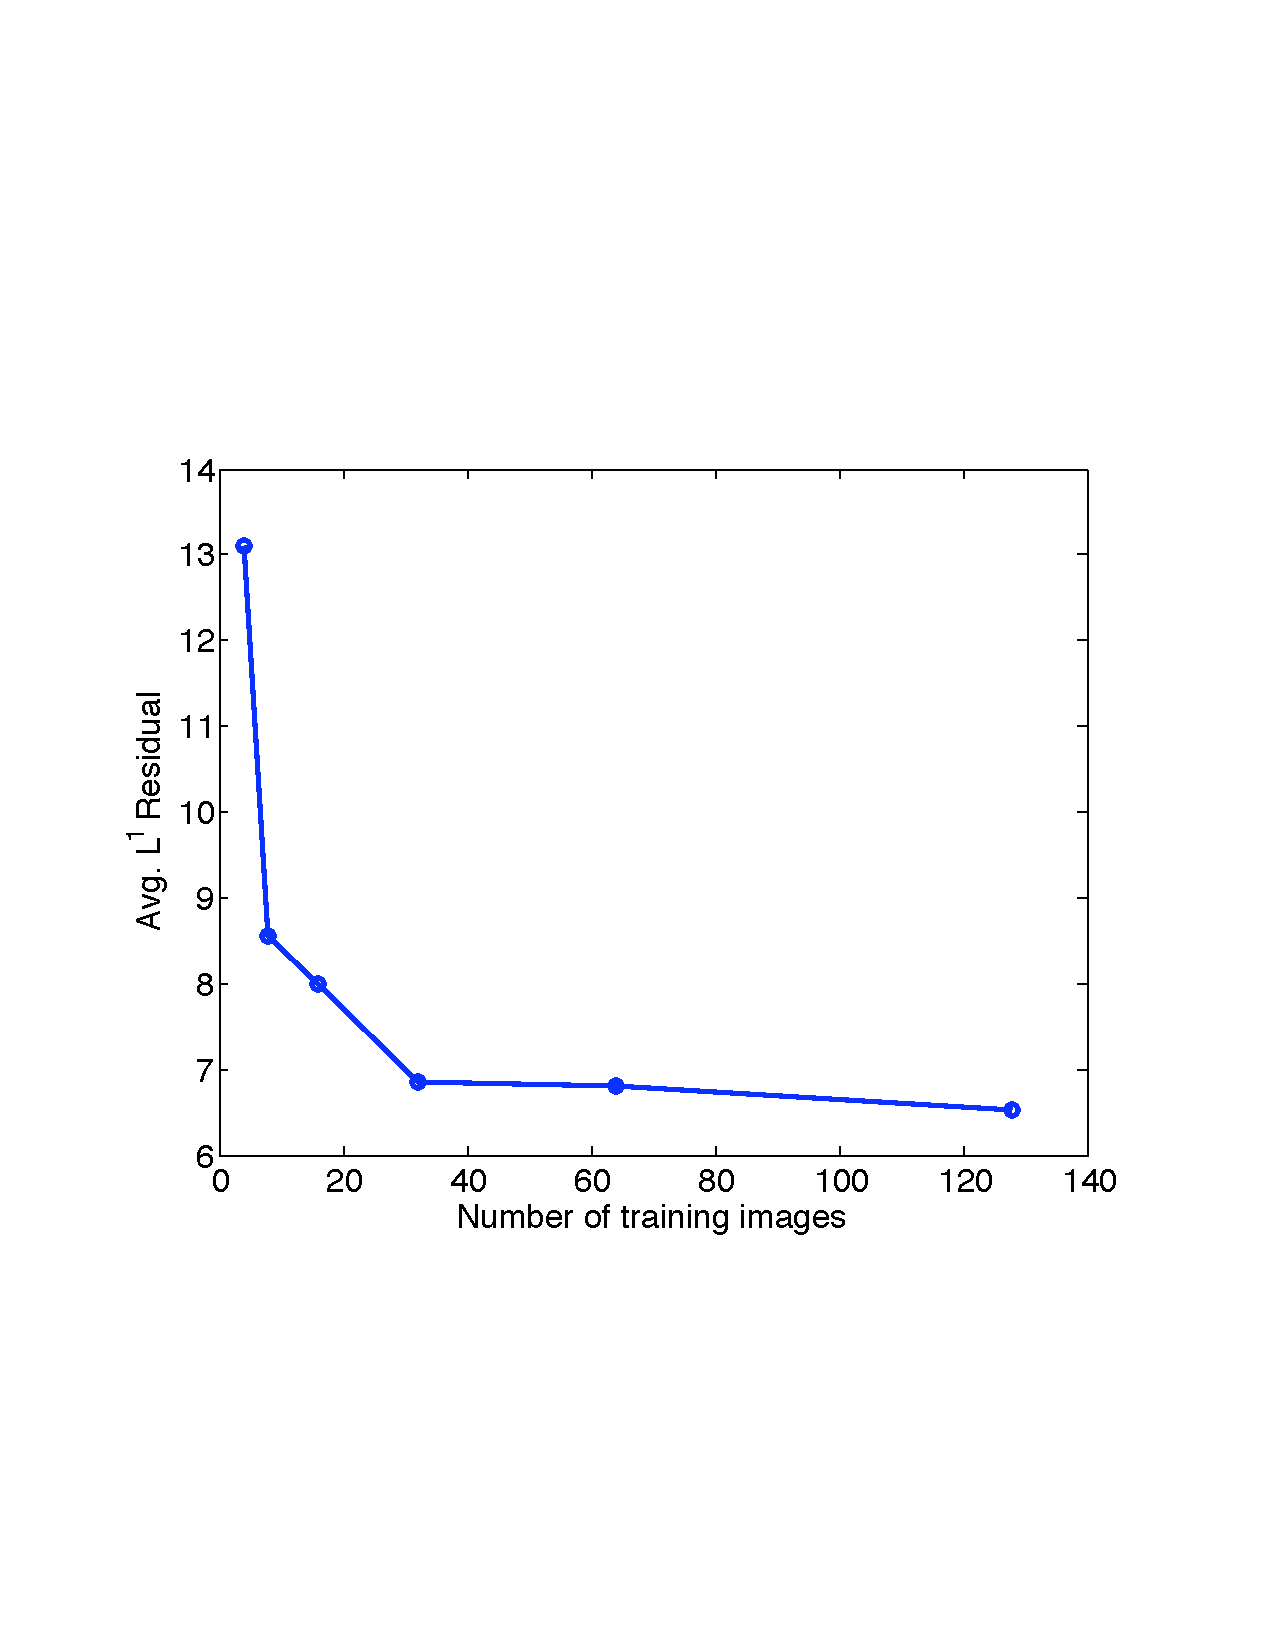
\includegraphics[height=2in]{figures_pami/illum_results/granularity_sunset.pdf} \\
(a) Coverage & (b) Granularity
\end{tabular}
\caption{\small{\bf Study of sufficient illuminations.} The average $\ell_1$
registration residual versus different illumination training sets. }
\label{fig:illumination-sufficiency}
\end{figure}

In the plot for the coverage experiment, Figure
\ref{fig:illumination-sufficiency}(a), two plateau regions can be observed: one
is after 4 rings and one is after 10 rings. The first four rings represent the
typical frontal illuminations, which are present in most public face data sets;
however, the residual does not stabilize until after 10 rings, which include
some illuminations from the back of the subject. This suggests that although
the frontal illuminations account for most of the illumination on the face,
some illuminations from the back are needed in the training set to represent
images with illumination coming from all directions.  In the plot for the
granularity experiment, Figure \ref{fig:illumination-sufficiency}(b), the
residual reaches a plateau after four divisions, corresponding to a total of 32
illuminations. Motivated by the results from the above two experiments, the
illumination area covered by the first 10 rings is partitioned into a total of
38 cells, whose layout is shown in Figure \ref{fig:illumination-patterns}(b).
For large scale experiments, the same set of illuminations just described is
used for capturing gallery images for all of the subjects.\footnote{It is
possible that with further experimentation a reduced set of illuminations can
be found that performs as well or better.}

Figure \ref{fig:sample_training_images} shows the full set of 38 training images 
for an example subject:
\begin{figure}[h]
\caption{\small Example of the set of 38 training images for one subject}
\centering
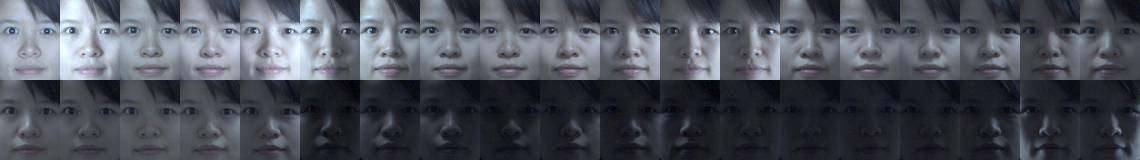
\includegraphics[width=\textwidth]{figures_pami/training.png}
\label{fig:sample_training_images}
\end{figure}

\section{Tests on Public Databases}\label{sec:multipie} In this section and the
next section, comprehensive experiments are conducted on large-scale face
databases to verify the performance of our face recognition pipeline.  The
largest public face database available that is suitable for testing the
$\ell_1$-minimization based pipeline, the CMU Multi-PIE data set, is used for
the first experiment.  One shortcoming of the CMU Multi-PIE database for this
purpose is that there is no separate set of test images taken under natural
illuminations; it is necessary to choose subsets of pictures taken in a lab
setting to use for testing and training.  To challenge the algorithm, only a
small set of illuminations for the training set is chosen, yet all
illuminations are included in the testing set. In the following section, the
performance the $\ell_1$-minimization based pipeline is tested on a face
data set that is collected by the projector-based acquisition system. The goal
for this experiment will be to show that with a sufficient set of training
illuminations for each subject, the algorithm indeed works stably and robustly
with practical illumination, misalignment, pose, and occlusion, as already
indicated by the experiment shown in Figure \ref{fig:promo} (bottom).

CMU Multi-PIE provides the most extensive test set among public
data sets. This database contains images of 337 subjects across
simultaneous variation in pose, expression, and illumination.
Of these 337 subjects, all of the 249 subjects 
in Session 1 are used as the training set. The remaining 88 subjects are
treated as ``impostors,'' or invalid images. For each of the
249 training subjects, frontal images are used with 7 frontal
illuminations,\footnote{They are illuminations
$\{0,1,7,13,14,16,18\}$ of \cite{Gross2008-FGR}. For each
directional illumination, the ambient-illuminated
image 0 is subtracted.} taken with neutral expression. As suggested by the
work of \cite{Georghiades2001-PAMI}, these extreme
frontal illuminations are used in the hope that they would linearly
represent other frontal illuminations well. For the test set,
all 20 illuminations from Sessions 2-4, which were
recorded over a period of several months, were used. The data set is
challenging due to the large number of subjects, and due to
natural variation in subject appearance over time.
Table \ref{tab:MultiPIE-recognition2} shows the performance of the
recognition pipeline on each of the 3 testing sessions. The pipeline
achieves recognition rates above $90\%$ for all three sessions.
For the test images, the iterative alignment algorithm was initialized
automatically via the Viola and Jones' face detector. To
demonstrate that the sparse representation based recognition
step is indeed beneficial even when there are no impostors, 
results for recognition based only on the alignment
error residuals (i.e. $S=1$) are shown in row 1.

\begin{table}
\caption{Recognition rates on the Multi-PIE database for
Algorithm 1 and \cite{Yang2010-CVPR}.}
\centerline{
\begin{tabular}{|c|c|c|c|c| }
\hline
Recognition rate & Session 2 & Session 3 & Session 4  \\
\hline
{Alg. 1, $S=1$} & 90.7\% & 89.6\% & 87.5\% \\
\hline
{Alg. 1} & 93.9\% & 93.8\% & 92.3\% \\
\hline
{Alg. 1 with improved window} & 95.0\% & {\bf 96.3}\% & {\bf 97.3}\% \\
\hline
\cite{Yang2010-CVPR} & {\bf 95.2}\% & 93.4\% & 95.1\% \\
\hline
\end{tabular}
\label{tab:MultiPIE-recognition2} }
\end{table}

\newcommand{\tempwidth}[0]{0.9in}
\begin{figure}
\centering
{
\begin{tabular}{@{}c@{}c@{}c@{}c@{}c@{}c@{}}
\hspace{-2mm}
\includegraphics[width=\tempwidth,clip=true]{figures_pami/multipie_failed/079_01_01_051_08.png}  &
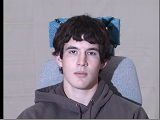
\includegraphics[width=\tempwidth,clip=true]{figures_pami/multipie_failed/111_01_01_051_08.png}  &
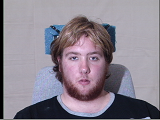
\includegraphics[width=\tempwidth,clip=true]{figures_pami/multipie_failed/196_01_01_051_08.png}  &
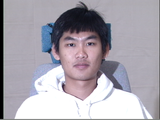
\includegraphics[width=\tempwidth,clip=true]{figures_pami/multipie_failed/130_01_01_051_08.png}  &
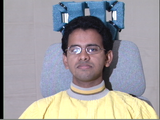
\includegraphics[width=\tempwidth,clip=true]{figures_pami/multipie_failed/163_01_01_051_08.png}  &
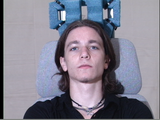
\includegraphics[width=\tempwidth,clip=true]{figures_pami/multipie_failed/175_01_01_051_08.png} \\
\hspace{-2mm}
\includegraphics[width=\tempwidth,clip=true]{figures_pami/multipie_failed/079_02_01_051_08.png}  &
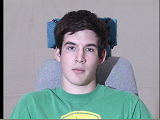
\includegraphics[width=\tempwidth,clip=true]{figures_pami/multipie_failed/111_02_01_051_08.png}  &
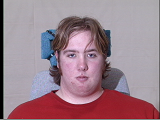
\includegraphics[width=\tempwidth,clip=true]{figures_pami/multipie_failed/196_02_01_051_08.png}  &
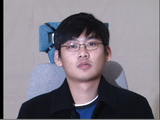
\includegraphics[width=\tempwidth,clip=true]{figures_pami/multipie_failed/130_02_01_051_08.png}  &
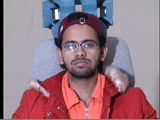
\includegraphics[width=\tempwidth,clip=true]{figures_pami/multipie_failed/163_02_01_051_08.png}  &
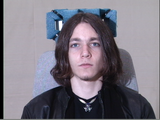
\includegraphics[width=\tempwidth,clip=true]{figures_pami/multipie_failed/175_02_01_051_08.png} \\
\hspace{-2mm}(a) & (b) & (c) & (d) & (e) & (f) 
\end{tabular}
}
\caption{\small{\bf Representative failures from Multi-PIE}. {\bf Top row:} Training from Session 1. {\bf Bottom row:} Test images from Session 2. Due to changes in hair, glasses, beard, or pose, our alignment fails on these subjects regardless of test image illumination.}
\label{fig:failed-examples}
\end{figure}
\subsection{Improving the Sampling Window}
The proposed recognition algorithm's errors are mostly caused by a few subjects who
significantly changed their appearances between sessions (such
as hair, facial hair, and eyeglasses). Some representative
examples are shown in Figure \ref{fig:failed-examples}. For those subjects, alignment and recognition fail on
almost all test illuminations.
\begin{figure}[b]
\centering
{
\begin{tabular}{@{}cc@{}}
\includegraphics[trim=1.9in .7in 1.9in .5in, clip, height=1.8in]{figures_pami/example.png} &
\includegraphics[trim=1.9in .7in 1.9in .5in, clip, height=1.8in]{figures_pami/example_new.png} \\
Default window. & Proposed window.
\end{tabular}
}
\caption{\small{\bf Choosing different sampling windows.}}
\label{fig:new-mask}
\end{figure}
Meanwhile, this observation also suggests that it might be possible to improve
the performance of the method by carefully choosing a face region which is less
affected by the above factors for recognition. In particular, since the
forehead region is likely to be affected by the change of hair style, it might
be helpful to replace the previously used $80 \times 60$ canonical frame with a
new window that better excludes the forehead.  Motivated by the observation
that in many cases the corners actually contain
background pixels, the two lower corners of the $80 \times 60$ canonical frame
are removed.  In addition, the resolution of the window is adjusted to keep $m$
approximately constant.  An example of the new window is shown in
Figure~\ref{fig:new-mask}.

\begin{table*}{5in}
\centering
\small
\caption{\small Recognition rates on the Multi-PIE database for
different pairings of alignment and recognition stages.}
\centerline{
\resizebox{5.4in}{!} {
\begin{tabular}{|c|c|c|c|c|c|c|c|c|c|c| }
\hline
\backslashbox{Rec.}{Align.}
& \multicolumn{3}{|c|}{Face Detector}
& \multicolumn{3}{|c|}{Manual}
& \multicolumn{3}{|c|}{Iterative Alignment}
\\
\hline
Session $\rightarrow$	& 2		&3			&4			& 2		&3			&4			& 2		&3			&4		\\
\hline
NS	& 30.8\%	& 29.4\%	& 24.6\%	& 77.6\%	& 74.3\%	& 73.4\%	& 84.5\%	& 82.3\%	& 81.4\% \\
\hline
NN	& 26.4\%	& 24.7\%	& 21.9\%	& 67.3\%	& 66.2\%	& 62.8\%	& 73.5\%	& 69.6\%	& 69.3\% \\
\hline
LDA	& 5.1\%		& 5.9\%		& 4.3\%		& 49.4\%	& 44.3\%	& 47.9\%	& 91.0\%	& 89.9\%	& 88.1\% \\
\hline
LBP	& 39.9\%	& 38.1\%	& 33.9\%	& 93.3\%	& 91.2\%	& 92.9\%	& {\bf 95.2\%}	& {\bf 94.7\%}	& {\bf 93.5\%} \\
\hline
SRC	& -- & -- & -- & -- & -- & -- & 93.9\%	& 93.8\%	& 92.3\% \\
\hline
\end{tabular}
}
\label{tab:MultiPIE-recognition} }
\end{table*}

Table \ref{tab:MultiPIE-recognition2} shows that the recognition rates on
Multi-PIE indeed increase with this new window. In addition, Figure
\ref{fig:failed-examples}(a), (b), and (c) illustrate three representative
subjects for which the recognition rates of the algorithm are significantly
boosted with the new window. However, it should be mentioned that the best
choice of the window may be specific to the data set and there is not a simple
guideline to follow. For example, although the new window performs better on
Multi-PIE, the same window does not help at all on the new database to be
introduced in the next section. This is because most of the training and
testing images in our database are taken on the same day so the variation in
hair style is very small. Hence, excluding the forehead part may actually
result in loss of useful discriminative information.

\subsection{Comparison to Existing Work}

The performance of the proposed recognition pipeline is first compared to
\cite{Yang2010-CVPR}. In \cite{Yang2010-CVPR}, the initial registration is
obtained from manually selected outer eye corners. Then, a supervised
hierarchical sparse coding model based on local image descriptors is trained,
which enjoys certain translation invariant properties. With the same training
and testing sets, \cite{Yang2010-CVPR} is able to handle the remaining
misalignment and achieves state-of-the-art performance on the CMU Multi-PIE
database.  Table~\ref{tab:MultiPIE-recognition2} shows that the proposed
algorithm achieves similar or better performance on different sessions of
Multi-PIE.

% Classical algorithms
To examine the effect on recognition rate of the iterative alignment algorithm
separately from the SRC-based recognition stage, in this experiment it is
combined with baseline linear-projection-based algorithms, such as Nearest
Neighbor (NN), Nearest Subspace (NS) \cite{Lee2005-PAMI}, and Linear
Discriminant Analysis (LDA) \cite{Belhumeur1997-PAMI}.\footnote{We do not list
results on PCA \cite{Turk1991-CVPR} as its performance is always below that of
Nearest Subspace.} Since these recognition algorithms assume pixel-accurate
alignment, they are not expected to work well if the test image is not well
aligned with the training. In Table~\ref{tab:MultiPIE-recognition}, recognition
rates are computed for these classical algorithms with three types of testing
image alignment: 1.\ alignment from the Viola and Jones' detector, 2.\
alignment via manually selected outer eye corners,\footnote{Two manually
clicked points are sufficient to define a similarity transformation. All of the
experiments in this section are carried out with similarity transformations.}
and 3.\ the output of the iterative alignment algorithm. The performance drop
of the LDA algorithm on Multi-PIE reported here seems to agree with that
reported already in \cite{Gross2008-FGR}.  All of the classical algorithms
benefit greatly from being paired with the proposed iterative alignment
algorithm.

% LBP
The performance of the pipeline is next compared to Local Binary Patterns (LBP)
\cite{Ahonen2006-PAMI}, a local appearance descriptor which is able to capture
fine details of facial appearance and texture.  Due to its robustness to
variations in illumination, facial expression, aging and other changes, LBP has
achieved the state-of-the-art face recognition performance in the scenario when
only one sample per person is used for training \cite{Tan06facerecognition}. In
this section, the same steps as in \cite{Ahonen2006-PAMI} are followed to
construct an LBP descriptor for each training and testing sample. The $80\times
60$ face region is first divided into a regular $10\times 10$ grid of cells,
each of size $8\times 6$ pixels. Within each cell, the histogram of 59 uniform
binary patterns is then computed, where the patterns are generated by
thresholding 8 neighboring pixels in a circle of radius 2 using the central
pixel value. Finally, the local histograms are concatenated to produce the
global descriptor vector. As suggested in \cite{Ahonen2006-PAMI}, the
recognition is performed using a nearest neighbor classifier with chi square
distance as the distance measure. Recognition rates with the
same three types of alignment input as before are reported.

As shown in Table~\ref{tab:MultiPIE-recognition}, although LBP
achieves competitive recognition rates given manually aligned
training and testing samples, demonstrating its robustness to
moderate misalignment, it still benefits from using the output
of the iterative alignment algorithm as the input. In addition,
like the other classical algorithms, the performance of LBP
degrades dramatically if it is applied directly to the output
of a face detector. This is notable given that LBP is often
applied without any special alignment in practice. Finally, we
attribute the improvement in performance of LBP over SRC in
this experiment to its robustness to illumination components
that cannot be linearly interpolated by the training set.

Although the SRC algorithm is not designed for recognition when there is only a
single gallery image per user, its performance with LBP is compared within this
setting for completeness. This experiment uses the FERET data set
\cite{phillips1998feret}, which contains five standard partitions: `fa' is the
gallery containing 1196 frontal images of 1196 subjects, and `fb', `fc', `dup1'
and `dup2' are four sets of probe images. The testing sets differ from the
training in facial expression (`fb'), illumination (`fc'), aging (`dup1') and
long aging (`dup2'). In fact, except for `fb', there are significant changes of
illumination in all the other three test sets.  For the training set, each
original is again cropped to an $80\times 60$ window using manually marked eye
coordinates \cite{Deng2010-PR} and normalized to unit $\ell_2$ norm.  In
Table~\ref{tab:FERET-recognition}, the performance of the SRC-based pipeline is
computed for the four test sets, with input directly obtained from the Viola
and Jones' detector.  The performance of LBP with the same three types of input
as before is reported: the letters $d$, $m$, and $i$ are used to
indicate face detector, manual alignment, and the iterative alignment
algorithm, respectively.

As expected, the proposed algorithm does not perform well except for
`fb', in which the illumination is similar to the training and
the mere variation in facial expression is handled well by the
sparse error model. For the other three test sets, the
algorithm fails because the illumination changes and other
variations seriously violate the assumptions of the method.
This also explains why LBP performs worse with iterative
alignment algorithm, compared to manual alignment. On the other
hand, while LBP achieves the best recognition rates given
manually aligned training and testing samples, its performance
degrades drastically when the input is obtained directly from
the face detector. It is also worth noting that similar poor
performance of LBP, as well as other descriptors, has been
observed on the Labeled Face in the Wild (LFW) database, where
the training is uncontrolled and limited and the input is
directly obtained from the face detector \cite{Wolf2008-ECCV}.
\begin{table}
\caption{Performance on single gallery image FERET data set.}
\centerline{
\begin{tabular}{|c|c|c|c|c| }
\hline
Recognition rate \% & fb & fc & dup1 & dup2 \\
\hline
$LBP_d$ & 54.8 & 10.3 & 29.8 & 19.8 \\
\hline
$LBP_m$ & {\bf 96.6} & {\bf 58.8} & {\bf 71.6} & {\bf 61.5} \\
\hline
$LBP_i$ & 94.5 & 42.8 & 46.5 & 21.1 \\
\hline
{Alg. 1} & 95.2 & 28.4 & 46.1 & 20.3 \\
\hline
\end{tabular}
\label{tab:FERET-recognition} }
\end{table}

All of these experimental results confirm that
both illumination and alignment need to be simultaneously handled
well in order to achieve accurate face recognition, even when there is
no obvious occlusion or corruption in the test.

\subsection{Subject Validation}

The next experiment tests the algorithms' ability to reject invalid images of the
88 subjects not appearing in the training database. As
mentioned before, the \emph{sparsity concentration index} (SCI)
is used as the outlier rejection rule. Given the sparse
representation $\x$ of a test image with respect to $K$
training classes, the SCI measures how concentrated the
coefficients are on a single class in the data set and is
defined as in \cite{Wright2009-PAMI}:
\begin{displaymath}
\textup{SCI}(\x) \doteq \frac{K \cdot \max_i \|\delta_i(\x)\|_1 /
\|\x\|_1 - 1}{K - 1} \in [0,1] .
\end{displaymath}
It is easy to see that if $\textup{SCI}(\x) = 1$, the test
image is represented using images from one single subject
class; if $\textup{SCI}(\x) = 0$, the coefficients are spread
evenly over all classes. Thus, a threshold $t \in
[0,1]$ can be chosen for the proposed method and accept a test image as valid
if $\textup{SCI}(\x) \geq t$, and otherwise reject it as
invalid. This classifier is compared to classifiers based on
thresholding the error residuals of NN, NS, LDA, and LBP.
\begin{figure}[t]
{
\centerline{
\begin{tabular}{@{}cc@{}}
\includegraphics[height=2.5in]{figures_pami/pami_roc_revision2} &
\includegraphics[height=2.5in]{figures_pami/pami_roc2} \\
(a) & (b) \\
\end{tabular}
}}
\caption{\small {\bf ROC curves} for subject validation on Multi-PIE database,
(a) for all algorithms with iterative alignment, and
(b) for the classical algorithms with manual alignment (indicated by a subscript ``m'').}\label{fig:roc-multipie}
\end{figure}

Figure \ref{fig:roc-multipie} plots the receiver operating characteristic (ROC)
curves, which are generated by sweeping the threshold $t$ through the entire
range of possible values for each algorithm.\footnote{Rejecting invalid images
not in the entire database is much more difficult than deciding if two face
images are the same subject. Figure \ref{fig:roc-multipie} should not be
confused with typical ROC curves for face similarity, e.g.
\cite{PhillipsP2007}.} On the left it can be seen that the SCI based
recognition approach significantly outperforms the other algorithms, including
LBP, even when all algorithms are coupled with the proposed iterative
alignment.  In the right plot we again see that classical algorithms, and even
LBP, are very sensitive to alignment.  Similar contrasts between the SRC
algorithm and baseline algorithms were also observed in \cite{Wright2009-PAMI},
though on much smaller data sets.

\subsection{Recognition with Synthetic Random Block Occlusion}

Next, the robustness of the $\ell_1$-norm based
algorithm to synthetic occlusion is tested further. 
Various levels of
occlusion from 10\% to 50\% are simulated by replacing a randomly located
block of the face image with an image of a baboon, as shown in
Figure~\ref{fig:multipie-occ-rec}. In this experiment, to avoid
any other factors that may contribute to extra occlusion of the
face (such as the change of hair style), illumination
10 from Session 1\footnote{This is the same session as the
training set.} is chosen for the test set. The rest of the experimental setting
remains unchanged. The table in
Figure~\ref{fig:multipie-occ-rec} shows that the proposed algorithm is
indeed capable of handling a moderate amount of occlusion. For
example, at 20\% occlusion, the algorithm still achieves 94.9\%
recognition rate.

\renewcommand{\tempwidth}{0.2\textwidth}
\begin{figure}
\centering
\begin{tabular}{@{}c@{}c@{}c@{}c@{}c@{}}
\includegraphics[width=\tempwidth,clip=true]{figures_pami/multipie_occ/occ10.png} &
\includegraphics[width=\tempwidth,clip=true]{figures_pami/multipie_occ/occ20.png} &
\includegraphics[width=\tempwidth,clip=true]{figures_pami/multipie_occ/occ30.png} &
\includegraphics[width=\tempwidth,clip=true]{figures_pami/multipie_occ/occ40.png} &
\includegraphics[width=\tempwidth,clip=true]{figures_pami/multipie_occ/occ50.png}  \\
\end{tabular}
{
\begin{tabular}{|c|c|c|c|c|c| }
\hline
Percent occluded & 10\% & 20\% & 30\% & 40\% & 50\%  \\
\hline
Recognition rate & 99.6\% & 94.9\% & 79.6\% & 46.5\% & 19.8\% \\
\hline
\end{tabular}
}
\caption{\small{\bf Recognition under varying level of random block occlusion.}
Examples of occluded test images with occlusion
level from 10\% to 50\% (left to right). The $\ell_1$-minimization based method maintains high recognition rates up to 30\%
occlusion, as shown in the table.}
\label{fig:multipie-occ-rec}
\end{figure}

\subsection{Recognition with Pose and Expression} Although the performance of
the proposed 2D recognition pipeline does not model out-of-plane head pose
variation or changes in expression, the next experiment tests the performance
of the algorithm on a subset of the images from Multi-PIE with pose and
expression variation for the test set.  The experiment uses the same training
set as above, and a test set consisting of images from Session 2 with
$15^\circ$ pose, for all 20 illuminations. As expected, the recognition rate
drops, in this case to 78.0\%. The algorithm is also tested on images in
Session 3 with smiling expression, again for all 20 illuminations. The
recognition rate is 64.8\%.  Of course, there is some hope that the
performance of the method would be significantly improved if pose and expression
data were available in the training.

\section{Tests on Our Own Database}\label{sec:own-data} Using the training
acquisition system described in Section \ref{sec:illumination}, and shown in
Figure \ref{fig:system}, frontal views of 109 subjects {\em without eyeglasses}
under the 38 illuminations shown in Figure \ref{fig:illumination-patterns} have
been collected. To enable testing of the algorithm with more realistic and less
controlled test images, 935 images of the same subjects are taken with a
different camera under a variety of practical conditions.

\subsection{Necessity of Rear Illuminations} To determine how the set of
training illuminations affects the performance of the algorithm in practice,
the next experiment compares how well a few frontal illuminations can linearly
represent: 1. other frontal illuminations taken under the same laboratory
conditions, and 2. typical indoor and outdoor illuminations.  To this end, 7
illuminations per subject from the private database are used as the training
set.  The illuminations are chosen to be similar to the 7 illuminations used in
the previous experiment on Multi-PIE.\footnote{We use the illuminations $\{6,
9, 12, 13, 18, 21, 22\}$ shown in Figure \ref{fig:illumination-patterns}(b) to
mimic the illuminations $\{0, 1, 6, 7, 13, 14, 18\}$ in Multi-PIE.} The
algorithm is then tested on the remaining $24 - 7 = 17$ frontal illuminations
for all the subjects. The recognition rate is $99.8\%$, nearly perfect. We also
test the algorithm on 310 indoor images and 168 outdoor images of these
subjects taken under a variety of lighting conditions (category 1 and 2
specified below), similar to the one shown in Figure \ref{fig:promo}, and the
recognition rates for indoor and outdoor images drop down to $94.2\%$ and
$89.2\%$, respectively. This is a strong indication that frontal illuminations
taken under laboratory conditions are insufficient for representing test images
under typical indoor and outdoor illuminations.

\subsection{Large-Scale Test with Sufficient Training
Illuminations} The following experiment demonstrates the performance
of the $\ell_1$-minimization based pipeline under the conditions it
was designed for.  All 109 subjects and 38 illuminations
are used in the training, and 935 images of users taken under a variety of
practical illuminations and conditions are used for the test set. 
The test set has been manually partitioned into four main categories:
\begin{description}
\item[C1:] 310 \emph{indoor} images of 72 subjects without
    eyeglasses, frontal view
    (Fig.~\ref{fig:examples1-3}, row 1).
\item[C2:] 168 \emph{outdoor} images of 48 subjects without
    eyeglasses, frontal view
    (Fig.~\ref{fig:examples1-3}, row 2).
\item[C3:] 211 images of 32 subjects with \emph{eyeglasses}
    (Fig.~\ref{fig:examples1-3}, row 3).
\item[C4:] 246 images of 56 subjects with \emph{sunglasses}
    (Fig.~\ref{fig:examples4}).
\end{description}
\renewcommand{\tempwidth}{0.1667\textwidth}
\begin{figure}
\centering
\begin{tabular}{@{}c@{}c@{}c@{}c@{}c@{}c@{}}
\includegraphics[width=\tempwidth,clip=true]{figures_pami/uiuc_example/normal_indoor/DSC_1318.JPG} &
\includegraphics[width=\tempwidth,clip=true]{figures_pami/uiuc_example/normal_indoor/DSC_1521.JPG} &
\includegraphics[width=\tempwidth,clip=true]{figures_pami/uiuc_example/normal_indoor/DSC_1673.JPG} &
\includegraphics[width=\tempwidth,clip=true]{figures_pami/uiuc_example/normal_indoor/DSC_1732.JPG} &
\includegraphics[width=\tempwidth,clip=true]{figures_pami/uiuc_example/normal_indoor/DSC_1941.JPG} &
\includegraphics[width=\tempwidth,clip=true]{figures_pami/uiuc_example/normal_indoor/DSC_3766.JPG} \\
\includegraphics[width=\tempwidth,clip=true]{figures_pami/uiuc_example/normal_outdoor/DSC_1574.JPG} &
\includegraphics[width=\tempwidth,clip=true]{figures_pami/uiuc_example/normal_outdoor/DSC_1622.JPG} &
\includegraphics[width=\tempwidth,clip=true]{figures_pami/uiuc_example/normal_outdoor/DSC_1641.JPG} &
\includegraphics[width=\tempwidth,clip=true]{figures_pami/uiuc_example/normal_outdoor/DSC_3522.JPG} &
\includegraphics[width=\tempwidth,clip=true]{figures_pami/uiuc_example/normal_outdoor/DSC_3707.JPG} &
\includegraphics[width=\tempwidth,clip=true]{figures_pami/uiuc_example/normal_outdoor/DSC_3772.JPG} \\
\includegraphics[width=\tempwidth,clip=true]{figures_pami/uiuc_example/glasses/DSC_1397.JPG} &
\includegraphics[width=\tempwidth,clip=true]{figures_pami/uiuc_example/glasses/DSC_1532.JPG} &
\includegraphics[width=\tempwidth,clip=true]{figures_pami/uiuc_example/glasses/DSC_1556.JPG} &
\includegraphics[width=\tempwidth,clip=true]{figures_pami/uiuc_example/glasses/DSC_1585.JPG} &
\includegraphics[width=\tempwidth,clip=true]{figures_pami/uiuc_example/glasses/DSC_1688.JPG} &
\includegraphics[width=\tempwidth,clip=true]{figures_pami/uiuc_example/glasses/DSC_4035.JPG} \\
\end{tabular}
\caption{\small{\bf Representative examples of categories C1-C3}. One row for each category.}\label{fig:examples1-3}
\end{figure}
%\begin{figure}[h]
\begin{figure}
\centering
\begin{tabular}{@{}c@{}c@{}c@{}c@{}c@{}c@{}}
\includegraphics[width=\tempwidth,clip=true]{figures_pami/uiuc_example/sunglasses/DSC_1565.JPG} &
\includegraphics[width=\tempwidth,clip=true]{figures_pami/uiuc_example/sunglasses/DSC_3656.JPG} &
\includegraphics[width=\tempwidth,clip=true]{figures_pami/uiuc_example/sunglasses/DSC_3827.JPG} &
\includegraphics[width=\tempwidth,clip=true]{figures_pami/uiuc_example/sunglasses/DSC_4090.JPG} &
\includegraphics[width=\tempwidth,clip=true]{figures_pami/uiuc_example/sunglasses/DSC_4106.JPG} &
\includegraphics[width=\tempwidth,clip=true]{figures_pami/uiuc_example/sunglasses/DSC_4126.JPG} \\
\includegraphics[width=\tempwidth,clip=true]{figures_pami/uiuc_example/sunglasses_failed/DSC_1611.JPG} &
\includegraphics[width=\tempwidth,clip=true]{figures_pami/uiuc_example/sunglasses_failed/DSC_3528.JPG} &
\includegraphics[width=\tempwidth,clip=true]{figures_pami/uiuc_example/sunglasses_failed/DSC_3744.JPG} &
\includegraphics[width=\tempwidth,clip=true]{figures_pami/uiuc_example/sunglasses_failed/DSC_3995.JPG} &
\includegraphics[width=\tempwidth,clip=true]{figures_pami/uiuc_example/sunglasses_failed/DSC_4030.JPG} &
\includegraphics[width=\tempwidth,clip=true]{figures_pami/uiuc_example/sunglasses_failed/DSC_4095.JPG} \\
\end{tabular}
\caption{\small{\bf Representative examples of category C4}. Top row: Examples
where the overlapping blocks method of Section \ref{sec:overlapping_blocks}
succeeded. Bottom row: Examples where the overlapping blocks method
failed.}
\label{fig:examples4} 
\end{figure}
Viola and Jones' face detector is applied to these images and
the resulting detected faces are used as the 
initialization for the alignment stage.
Table~\ref{tab:UIUC-recognition} reports the performance of our
algorithm on each category.
Since the focus is on face
recognition rather than face detection, 
the errors do not include failures of the face
detector on some of the more challenging images.
The algorithm achieves higher than 95\%
recognition rates on categories 1-3. Furthermore, using the
full set of 38 illuminations indeed improves the performance of
the system under practical illumination conditions compared to
only using a small subset of 7 illuminations. However, the
performance dramatically drops when the faces are occluded by
various types of sunglasses, which could cover up to 40\% of
the entire face. Given the previous experimental results on
synthetic random block occlusions, and given that the
illuminations are more challenging, the result is not
surprising. The next subsection will show how additional
assumptions about the nature of the data can be used to improve 
the recognition performance.
\begin{table}[h]
\centering \caption{Recognition rates on a more realistic
private database.}
\begin{tabular}{|c|c|c|c|c| }
\hline
Test Category & C1 & C2 & C3 & C4  \\
\hline
\hline
Recognition Rate & 98.4\% & 95.8\% & 95.1\% & 40.9\% \\
\hline
\end{tabular}
\label{tab:UIUC-recognition}
\end{table}

\subsection{Improving the Performance with Occlusion Using Overlapping Blocks}
\label{sec:overlapping_blocks}
%
A traditional approach to improve the performance of face recognition under
severe occlusion is to use subregions instead the entire face as a whole. This
idea has been explored in many earlier works; see \cite{Pentland1994-CVPR,
Wright2009-PAMI} for examples. Since in most real-world cases the occlusion is
contiguous, it is reasonable to argue that a minority of the subregions are
likely to be affected by the occlusion. In this section, this idea is used
as motivation to 
partition the face into four overlapping blocks to better handle
occlusions caused by sunglasses. This scheme is illustrated in Figure~\ref{fig:occ-block}. Notice
that in this example three out of the four blocks are partially or almost
completely occluded. In the experiment, each block is of size $90\times 48$ and
covers about two-fifths of the entire face. The testing and training sets are
partitioned in the same way. 
Algorithm~\ref{alg:deformable-src} is then applied independently to each block,
and a sparse representation of the test image with respect to the training images
is computed, also independently for each block.
The recognition results for individual blocks are then aggregated by voting.

\begin{figure}
\centering
\includegraphics[width=4in]{figures_pami/occ_block.png}

\caption{\small{\bf Using overlapping blocks to tackle contiguous occlusion.}
(a) The test image, occluded by sunglasses. (b) The four overlapping blocks.
(c) The sparse representation is calculated after alignment for each block
independently. The red lines correspond to the test user's true identity. (d)
The true identity is successfully recovered by voting based on the SCI scores.}
\label{fig:occ-block} 
\end{figure}

The following experiment verifies that using the \emph{sparsity
concentration index} (SCI) scores for voting achieves a higher recognition rate
than the residual measure used in Algorithm~\ref{alg:deformable-src}, on
category 4 (sunglasses) of the database. The recognition rate is increased to
78.3\%, compared to 40.9\% obtained without this partition scheme. This provides
further evidence of the superiority of SCI for subject validation, since a
heavily occluded block can be regarded as an outlier for recognition and should
be rejected while voting.

Unfortunately, a major problem with this
approach is that occlusion cannot always be expected to fall within
 any fixed partition of the face image. Therefore, the
proposed scheme should only be viewed as an example which shows
that the performance under occlusion can be boosted by
leveraging local information of a face as well as global information. 
The investigation of improved models for occlusion, such as the {\em Markov random field} (MRF)
based algorithm presented in \cite{ZhouZ2009} and in Chapter \ref{chap:markov},
remains an interesting open research problem.

\section{Conclusion}\label{sec:conclusion}
The face recognition system described in this chapter leverages a
well-thought-out combination of existing ideas (iterative image alignment,
$\ell_1$-error function, SRC, and using projectors for illumination).  It is
capable of working with images taken under practical conditions and is
conceptually simple, well motivated, and competitive with state-of-the-art
recognition systems for access control scenarios.

The system achieves extremely stable performance under a wide range of
variations in illumination, misalignment, and even under small amounts of pose
and occlusion. Very good recognition performance is achieved on large-scale
tests with public data sets as well as more realistically captured probe images,
while using only frontal 2D images in the gallery and no explicit 3D face
model.  This system demonstrates that misalignment can be naturally handled
within the sparse representation framework.  The complete (from acquisition to
recognition) pipeline presented in this chapter forms the baseline reference
implementation for the rest of the work in this thesis.

This chapter further establishes the opportunity for further improvement of
recognition rates in the presence of occlusions by introducing more complicated
models for spatial continuity, such as Markov random fields.  This idea is
further addressed in Chapter \ref{chap:markov}.

